\documentclass[12pt]{article}
\usepackage[toc,page]{appendix}
\usepackage{amsmath}
\usepackage{afterpage}
\usepackage{cases}
\usepackage{amsfonts}
\usepackage{epsfig}
\usepackage{setspace}
\usepackage{pdflscape}
\usepackage{natbib}
\usepackage{placeins}
\usepackage{epigraph}
\usepackage{verbatim}
\usepackage{epigraph}
\usepackage{url}
\usepackage{lscape}
\usepackage{multirow}
\usepackage{longtable}
\usepackage{rotating}
\usepackage[table]{xcolor}
\usepackage[export]{adjustbox}
\usepackage{graphicx}
\usepackage{caption}
\usepackage{subcaption}
\usepackage{makecell}
\DeclareMathOperator*{\E}{\mathbb{E}}
\bibliographystyle{agsm}
\usepackage{tikz}

\usepackage[colorlinks=true, urlcolor=blue, citecolor = black]{hyperref}
\special{papersize=8.5in,11in}

\addtolength{\oddsidemargin}{-.6in} \addtolength{\evensidemargin}{-.6in}
\addtolength{\textwidth}{1.2in}

\addtolength{\topmargin}{-.6in} \addtolength{\textheight}{1.2in}

\makeatletter
\def\@sect#1#2#3#4#5#6[#7]#8{\ifnum #2>\c@secnumdepth
     \let\@svsec\@empty\else
     \refstepcounter{#1}\edef\@svsec{\csname the#1\endcsname. \hskip 0.4em}\fi
     \@tempskipa #5\relax
      \ifdim \@tempskipa>\z@
        \begingroup #6\relax
          \@hangfrom{\hskip #3\relax\@svsec}{\interlinepenalty \@M #8\par}%
        \endgroup
       \csname #1mark\endcsname{#7}\addcontentsline
         {toc}{#1}{\ifnum #2>\c@secnumdepth \else
                      \protect\numberline{\csname the#1\endcsname}\fi
                    #7}\else
        \def\@svsechd{#6\hskip #3\relax  %% \relax added 2 May 90
                   \@svsec #8\csname #1mark\endcsname
                      {#7}\addcontentsline
                           {toc}{#1}{\ifnum #2>\c@secnumdepth \else
                             \protect\numberline{\csname the#1\endcsname}\fi
                       #7}}\fi
     \@xsect{#5}}
\makeatother

\makeatletter
\renewcommand{\section}{\@startsection{section}{1}{0mm}{-\baselineskip}{0.20\baselineskip}{\centering\normalfont\normalsize\scshape}}
\renewcommand{\subsection}{\@startsection{subsection}{2}{0mm}{-\baselineskip}{0.25\baselineskip}{\raggedright\normalfont\normalsize\scshape}}
\renewcommand{\subsubsection}{\@startsection{subsubsection}{3}{0mm}{-\baselineskip}{0.25\baselineskip}{\raggedright\normalfont\small\scshape}}
\def\@begintheorem#1#2{\trivlist \item[\hskip \labelsep{\bf #1\ #2:}]\it}
\makeatother

\makeatletter
\def\monthname{\ifcase\month\or
January\or February\or March\or April\or May\or June\or July\or August\or
September\or October\or November\or December\fi} \makeatother

\renewenvironment{epigraphwidth}{\setlength{13.5cm}}

\renewcommand{\thesection}{\Roman{section}}
\renewcommand{\thesubsection}{\Alph{subsection}}

\renewcommand{\thesubfigure}{\Alph{subfigure}}

\renewenvironment{abstract}
 {\begin{center}\normalsize\textsc{}%
 \end{center}\begin{quote}\normalsize}
 {\end{quote}}


\renewcommand{\appendix}{\footnotesize\parindent 0cm\setlength{\parskip}{\medskipamount}\setcounter{equation}{0}%
\renewcommand{\theequation}{A.\arabic{equation}}}

\newtheorem{theorem}{\small\sc Theorem}[section]
\newtheorem{proposition}{\small\sc Proposition}[section]
\newtheorem{assumption}{\small\sc Assumption}[section]
\newtheorem{lemma}{\small\sc Lemma}[section]
\newtheorem{corollary}{\small\sc Corollary}[section]
\newtheorem{hypothesis}{\small\sc Hypothesis}

\usepackage{chngcntr}


\newcommand{\indep}{\perp\!\!\!\!\perp}

\begin{document}
\begin{titlepage}
\vspace*{0.2cm}

\setcounter{page}{0}

\vskip 10pt
  \begin{center}%
    {\Large \sc Online Activism and Dyadic Representation: \\ Evidence from the UK E-Petition System \\
   {\small Short title: \emph{Online Activism and Dyadic Representation}}\\
   \vspace{.25cm}
{\small    \emph{Forthcoming in Legislative Studies Quarterly}}
   \vspace{.5cm} \par}%

    \vskip 1em%
    {\large
     \lineskip .75em%
      \begin{tabular}[t]{c}%
       Jack Blumenau 
      \end{tabular}  
\vskip 1em 
\textsc{University College London}
\par}%
      \vskip 2.5em%
  \end{center}\par

 \vskip 3.0em
\begin{center} \textsc{Abstract} \end{center}

\begin{abstract}


By making it easier for citizens to communicate their preferences, online forms of political participation have the potential to strengthen the representational link between politicians and voters. However, we know little about the effects of online advocacy on politicians' behaviour. Using new data from an e-petition system in the UK, I show that support for a petition among a Member of Parliament's constituents is associated with a substantial increase the probability that the MP advocates for the petition in parliamentary debate, even when compared to MP behaviour in counterfactual non-petition debates which focus on the same policy issues. However, MP responsiveness is conditioned both by party discipline and electoral competition. These findings have important implications for our understanding of dyadic representation in parliamentary systems.


\end{abstract}

Key words: Representation; Petitions; Parliamentary Debate; House of Commons \\~\\

Word count: 9995

\vfill
  \footnoterule
    {\footnotesize
\noindent 	
	This version: \monthname \ \number\year. \\ I thank Ben Lauderdale, Tom O'Grady, Cristina Leston Bandeira, and three anonymous reviewers for providing helpful comments. I am also grateful to participants at the LSE Political Behaviour and LSE Methodology seminars, the Oxford DPIR research colloquium, and EPSA and MPSA 2017. I also thank Roberta Damiani for excellent research assistance. This work was supported by the Economic and Social Research Council (grant number: ES/N016297/1).
	



\noindent\footnotesize

}
\end{titlepage}

\newpage
\setcounter{page}{1} \addtolength{\baselineskip}{0.5\baselineskip}

\noindent Normative theories of democratic representation suggest that, when viewed as delegates, politicians should advance the preferences of their constituents \citep{pitkin1967concept}. In single-member district (SMD) electoral systems, a key concern is whether legislators' actions reflect the specific views of their districts -- a concept usually described as ``dyadic'' representation \citep{weissberg1978collective}. Indeed, the idea that SMD-systems incentivise responsiveness to local concerns is commonly cited as one of their central virtues \citep{norris2001twilight, carey2011electoral}. However, a central dilemma for reelection-seeking politicians is that acquiring information on the preferences of voters can be difficult and costly. This can have pernicious effects, for even when politicians have incentives to adapt their behaviour to reflect constituents' preferences, a paucity of information will mean that politicians' knowledge of such preferences may be biased \citep{norris2004parties,broockman2018bias}; that responsiveness will be limited \citep{stimson1995dynamic}; and that the quality of democratic representation is likely to suffer \citep[518]{mansbridge2003rethinking}. Put bluntly, it is hard to do what the voters want if you do not know what it is that the voters want you to do. 

The growth of online political activity therefore represents an important change to the information environment faced by politicians. By lowering the costs of acquiring political knowledge and giving citizens new mechanisms for communicating with their representatives, the internet has the potential to improve the informational link between politicians and voters. For some scholars, this promises to strengthen representation and ``enrich democracy'' \citep[11]{coleman2009internet}. However, despite these claims, we lack empirical evaluations of whether new online forms of political expression have had tangible effects on the quality of dyadic responsiveness. This paper helps to fill this gap. 

In particular, I investigate the effects on dyadic representation of one popular form of online democratic engagement: government-sponsored electronic petition (e-petition) systems. Taking the UK as a case study of the effectiveness of these systems, I argue that e-petitions represent a valuable source of information on constituent preferences for reelection-seeking Members of Parliament (MPs). The SMD electoral system used for Westminster elections creates incentives for MPs to cater to their constituents \citep{cain1984constituency} and although these incentives may be weaker than in some other systems \citep{carey1995incentives}, recent evidence suggests that voters in the UK are more supportive of MPs who have strong local links with the constituency \citep{campbell2019friends}; who dedicate more time to constituency issues \citep{vivyan2016house}; and who demonstrate greater independence from the party line \citep{vivyan2012voters, campbell2019legislator}. However, due to a paucity of polling information at the local level in the UK, MPs typically learn about constituent preferences through imperfect signals -- emails, letters, face-to-face interaction, social media, etc -- which makes it difficult to form accurate judgements of constituency opinion, and potentially inhibits legislator responsiveness. 

The petition data I study, by contrast, provides MPs with useful information for evaluating the strength of constituency opinion across a variety of issues. E-petitions are publicly available on a dedicated government website where anyone can sign by providing their name, email address and postcode. The system is popular: UK e-petitions accumulated more than 50 million signatures between 2015 and 2019, and petition-signing is the second most popular form of political activity (after voting) in the UK, with nearly 30\% of adults reporting signed e-petitions each year \citep{hansard2018audit}. Critically, the e-petitions website also presents signature counts for each petition at the level of parliamentary constituencies. Legislators can therefore observe the local strength of support for each petition and use this information to guide their actions in ways that are likely to be electorally rewarding, and in so doing may improve the representation of constituent interests in the policy process.

Politicians in parliamentary systems such as the UK, even when sufficiently informed about constituent preferences, may be prevented from demonstrating responsiveness to local demands by party leaders who wield strong powers of party discipline and agenda control. As Cain et al. (\citeyear[217]{cain1987personal}) suggest, an inherent tension in SMD parliamentary systems is that ``electoral rules create incentives for a personal vote and legislative rules deny representatives the opportunity to establish it." However, the petition system in the UK also provides a venue for responding to that information which is generally not subject to control by party leaders: any e-petition that receives more than 100,000 signatures is considered for debate in parliament. MPs' speeches in the UK are significantly less constrained by party discipline than their voting decisions, and an MP's decision to participate in debate -- the main dependent variable of interest here -- also constitutes an important representative act, as making a speech in a debate of great local interest allows an MP to literally `speak up' for her constituents' interests. I therefore evaluate the dyadic relationship between UK MPs and constituents by examining patterns of participation in these petition debates.

The expectation I test is straightforward: MPs will be more likely to participate in debates on petitions marked by high levels of local support. However, if an MP already has a strong sense of which issues are important to her constituents, she might participate in a given petition debate even in the absence of the e-petition. An MP from an agricultural constituency, for example, will likely receive many signatures on agricultural petitions, will probably attend the relevant petition debates, but will probably also attend \emph{non-petition} agricultural debates. In such situations, the relationship between petitions signatures and debate behaviour will be confounded. While issues such as these cannot be entirely avoided when using observational data, I describe an empirical strategy which helps to reduce these concerns. Combining statistical topic models with a multilevel random-effects model, I show that MPs' responsiveness to constituent activism in petition debates differs from their behaviour in counterfactual non-petition debates that are otherwise very similar in terms of topical content. 

My argument and empirical analysis relates specifically to e-petition systems that are formally integrated into the broader political process, and so speaks less to non-governmental e-petition systems which have been the focus of study elsewhere \citep{halpin2018online}. Given that both academics and policymakers see e-petitions as a method for strengthening the representational bond between representatives and their constituents \citep{hough2012legislative, bochel2012petitions, kennedy2013electronic, committee2014epetitions}, the rapid adoption of these government-sponsored systems in many countries in recent years is perhaps unsurprising.\footnote{E-petition schemes have been introduced in the UK (\url{https://petition.parliament.uk}), the US (\url{https://petitions.whitehouse.gov}), Germany (\url{https://epetitionen.bundestag.de}), Canada (\url{https://petitions.ourcommons.ca}), Australia (\url{https://www.aph.gov.au/Parliamentary_Business/Petitions}), the Ukraine (\url{https://petitions.com.ua}), as well as in the European Parliament (\url{https://petiport.secure.europarl.europa.eu/petitions}) and in many local government settings \citep{hough2012legislative}.} However, the empirical literature on e-petitions has largely been limited to descriptive evidence of the petitioning process, with a focus on documenting the types of people who start \citep{wright2015populism} and sign \citep{jungherr2010political} e-petitions, the issue agendas petitions promote \citep{hersh2018postmaterialist}, the rate at which petitions grow \citep{yasseri2017rapid}, as well as perceptions of the effectiveness of such systems \citep{escher2017petitioning}. What is notably lacking from this literature is an assessment of the effects of these petitions on political representation within legislatures; something that I provide here.
 
In addition, the vast majority of research on dyadic representation has focused on the presidential system of the US \citep{miller1963constituency, kastellec2010public, krimmel2016gay}. While recent work suggests that dyadic responsiveness in parliamentary voting in the UK is non-zero \citep{hanretty2016dyadic}, such evidence is mostly limited to non-typical roll-call votes where no whip is imposed, or in rare instances where votes cut across party lines. Here, I go beyond roll-call votes and expand the range of activities examined to include MP participation in debates. Further, existing studies of dyadic representation in parliamentary systems either rely on demographic proxies for measuring constituency opinion \citep{hibbing1987accounting, soroka2009constituency,blidook2011constituency}, or are limited to evaluating the dyadic relationship on a small number of high-profile issues that are covered in national opinion polls \citep{hanretty2016dyadic}. As Stimson et al. (\citeyear{stimson1995dynamic}, 562) argue, ``while we, as scholars, rely solely on public opinion polls to do our work, politicians surely do not'', and so an additional value of studying e-petitions is that because petition signature counts are publicly available, they also offer a rare opportunity for researchers to observe the same indicators of constituency-demand as those observed by politicians.

I report three main results in the paper. First, MPs are substantially more likely to participate in debates relating to petitions signed by many of their constituents. Second, while this effect is robust to controlling for participation on topically-similar non-petition debates, MP responsiveness is clearly conditioned by both party discipline and electoral competitiveness. Finally, MPs not only \emph{participate} more in relevant debates, but are also more likely to use their speeches to \emph{express agreement} for e-petitions marked by stronger local support. Taken together, these findings suggest that e-democracy initiatives can significantly strengthen representational ties between citizens and politicians, but that the effects of such initiatives are also likely to be mediated by existing political incentives.


\section*{Information, Dyadic Representation, and Parliamentary Debate}

Positive accounts of representation suggest that reelection-seeking politicians will tailor their behaviour to satisfy the wishes of voters, either by taking positions that align with constituents' preferences, or by allocating attention to the most salient constituency-specific issues \citep{downs1957economic, mayhew1974congress, cain1984constituency, hall1996participation}.  Information is a central component of these theories \citep[516--520]{mansbridge2003rethinking}, as legislators are expected to infer the preferences of their constituents, and use this knowledge to guide their legislative decisions. However, legislators will only occasionally have access to high quality information to learn about the opinions of their constituents on particular policy issues. More commonly, legislators must rely on heuristics to evaluate the strength of local opinion towards policy: how much correspondence has the legislative office received? How prominent is the issue in local media? How often do constituents mention the issue ``on the doorstep''? It is therefore unsurprising that politicians invest significant resources in gathering information about constituent preferences \citep{maestas2003incentive}, and that even small changes in this information can translate into meaningful changes in legislative behaviour \citep{butler2017party, bergan2015call}.

For MPs in the UK, the value of e-petitions resides in the additional signal they offer about constituents' preferences. This information is marked by two important properties. First, e-petition signature counts are typically available at low geographic levels of aggregation. Locally-disaggregated information allows legislators to respond to the specific preferences of their constituents, which may differ from those of the population at large.  Such information is likely to be especially valuable in the UK, where constituency-specific polls are rare \citep{wring2016political, johnston2018exploring}. Constituency signature counts for each petition are made available on a centralised website, and this information is easy for MPs to access both in terms of the raw data and in the form of an interactive online map.\footnote{See appendix section \ref{app:eu_map} for an example} In addition, for petitions receiving more than 100 thousand signatures, the parliamentary Petitions Committee also provides this information directly to MPs by emailing them a spreadsheet of the signatures in each constituency \citep[48]{committee2014epetitions}. MPs clearly access this information, as they frequently refer to specific signature counts in the course of petition debates.\footnote{See appendix section \ref{app:petition_knowledge} for examples.}

Second, e-petitions tend to address a diverse set of topics, which contrasts with the limited range of issues considered by national opinion polls, and on which it is unlikely that MPs will always have strong prior understanding of constituent preferences. For instance, the petition calling on the government to ``Stop allowing immigrants into the UK''\footnote{\url{https://petition.parliament.uk/archived/petitions/106477}} is typical of the type of issue that might feature in UK election campaigns. By contrast, the petition that lobbied the government to ``Give the Meningitis B vaccine to ALL children''\footnote{\url{https://petition.parliament.uk/archived/petitions/108072}} addressed an issue that is not typically central to UK political debate, and where MPs were likely to have weaker intuitions about the importance of the issue to their constituents. E-petitions may therefore also be informative about constituent opinion on issues that have not previously been a part of the political agenda. Moreover, UK e-petitions feature both issues that represent crucial dividing lines in contemporary British politics,\footnote{See, for example, the petition on ``EU Referendum Rules triggering a 2nd EU Referendum'' \url{https://petition.parliament.uk/archived/petitions/131215}} and also `valence' issues on which most voters share a common preference.\footnote{See, for example, the petition entitled ``Prevent avoidable deaths by making autism/learning disability training mandatory'', \url{https://petition.parliament.uk/petitions/221033}} For issues that involve high-levels of voter disagreement, local petition signature counts can help MPs to learn about the balance of opinion on that issue among their constituents. For valence issues, signature counts may likewise be informative about the relative importance of the issue in the minds of voters. In either case, being attentive to constituency-specific petition support can help MPs to direct their legislative efforts in ways that are likely to appeal to their voters. 

Of course, the people who participate in online political activities may be different from those who participate offline -- something that is true of the people who sign e-petitions\footnote{See appendix section \ref{app:ecological}.} -- and so the number of signatures on a given petition will not enable an MP to accurately judge the absolute level of support for an issue among her constituents. However, MPs can still reasonably draw inferences about constituents' \emph{relative} issue priorities from petition signatures.  On the one hand, an MP could learn about the local salience of an issue by comparing the signature rate on a given petition in their constituency to the signature rate on that petition in other constituencies. Learning from these ``across-constituency'' comparisons simply requires the belief that petition-signers are similarly unrepresentative across different constituencies.  On the other hand, an MP could draw inferences by making comparisons between the signature rate in their constituency on one petition to the signature rate in their own constituency on other petitions. That there may be systematic differences between online activists and constituents in general is not problematic for making this type of ``within-constituency'' comparison, as such biases can be reasonably thought to be constant within constituencies across issues. 

Qualitative evidence suggests that MPs do in fact make comparisons both across constituencies, and within constituencies across petitions.\footnote{I report further examples in appendix section \ref{app:petition_knowledge}} For example, in a debate on a high-profile petition in 2017, one MP pointed out that a ``higher percentage of constituents from [my constituency] signed the petition than from any other constituency and I am proud to represent them today.''  \citep{lucas2017speech} Similarly, in a debate in 2018 another MP suggested that ``589 of my constituents have signed the petition, which is really high for my constituency.''  \citep{Hodgson2018speech} Overall, although the median petition-signer is unlikely to hold the same views as the median constituent, petitions can nevertheless be used to update legislators' beliefs about the best ways to allocate their time to different issues. As a consequence, measures of local petition support are likely to complement the diverse set of heuristics that MPs use to assess the strength of feeling for an issue in their constituency.

However, the informational value that e-petitions have in parliamentary systems may be mitigated by countervailing incentives to toe the party line. The combination of strong powers of party discipline and governmental agenda-control means that MPs in parliamentary systems will be less able to use their legislative voting behaviour to demonstrate responsiveness to local concerns than is the case for legislators in presidential systems \citep{carey2007competing}.  In the UK, for example, although defection in roll-call votes has increased in recent years, the strength of the party whip means that it remains relatively rare \citep{cowley_2015}, and voting records generally reflect partisan divisions rather than information about individual MP behaviour \citep{spirling2006uk}. While petitions may strengthen incentives for dyadic behaviour, party-discipline constraints in parliamentary systems may mean that MPs are unable to respond to such information. 

The UK petition system, however, provides MPs with an alternative mechanism for responding to petitioners' concerns. In particular, any petition that receives over 100,000 signatures nationally is considered for debate in parliament. Although the Petitions Committee has some discretion over which debates are scheduled, almost all petitions crossing the 100,000 threshold (as well as some slightly below it) have been debated.\footnote{Table \ref{tab:debated_petitions} in the appendix lists all \input{useful_numbers/n_petitions_wmin_hall.tex}petitions debated between June 2015 and February 2019.} These debates are attended by members of all political parties as well as the government minister responsible for the relevant department.  E-petition debates have become a high-profile part of the parliamentary week, both in the views of MPs themselves\footnote{As one MP puts it, ``These Monday afternoon debates are becoming something of a showpiece, and a bit box-office.'' \citep{grady2014speech}} as well as in terms of the amount of media coverage that is devoted to them.\footnote{See, for example, \href{https://www.bbc.co.uk/news/uk-politics-47772682}{``Article 50: MPs debate six-million signature petition'', \emph{BBC News}, 1st April 2019}, and \href{https://www.express.co.uk/news/politics/775463/High-heels-work-rule-MPs-debate-illegal}{``MPs debate bid to make it illegal to force women to wear high heels at work'', \emph{Daily Express}, 6th March, 2017}} 

How might we examine responsiveness in the context of these debates? Politicians may respond to new information about constituent preferences not only by changing their policy positions (as revealed by the votes they cast), but rather by shifting their legislative efforts towards issues that their constituents find most salient. As Hall (\citeyear[58]{hall1996participation}) suggests, constituency influence should not only operate on legislators' voting behaviour ``but on the intensities that they reveal in their decisions about when and to what extent they will participate in particular matters''. By allocating more of their time to the most pressing local issues, politicians demonstrate their willingness to address constituent concerns. In short, the decision to participate in a given debate can itself be a representational act.

Legislative debate is a useful arena for pursuing this type of strategy in the UK. First, parliamentary speeches are publicly visible acts that are widely covered in the UK media, and are easy to publicise to constituents. Speaking in parliament is also considered both by voters and MPs to be one of the most important roles that an MP performs \citep{campbell2014should}. Standing up and making a speech in a debate devoted to a petition which many of your constituents have signed allows the MPs to demonstrate that she has heard local concerns, and has given voice to those concerns in parliament. MPs frequently use parliamentary speeches to draw government attention to issues that are relevant to a certain constituency, or to request that a minister takes action relating to the case of a specific constituent. Indeed, the use of constituency-oriented language in parliamentary speech has increased dramatically in the Commons over the past 40 years \citep{blumenau2020parliamentary}.

In addition, the Petitions Committee provides direct links to both videos and transcripts of petition debates on the e-petition website, making it straightforward for MPs to promote their speeches and to claim credit for responding to petitioner concerns. While MPs cannot directly contact those constituents who signed the petitions -- the list of email addresses is not accessible to MPs -- they can, and do, report on their activity in petition debates on social media.\footnote{See, for example: 
\begin{itemize}
%\item Ian Blackford MP, ``I concluded debate on 2nd EU referendum petition. We respect others leave choice, but Scotland's view also counts. \texttt{https://t.co/KlDOEoa3p7?amp=1}'', 5 September, 2016, 8.14pm, Tweet.
\item Margaret Ferrier MP, ``I spoke yesterday during the South Korea dog meat trade debate - thanks to the public petitioners for securing it. \texttt{https://t.co/ZstsqOJkc9}'', 13 September 2016, 10.00am, Tweet.
\item Thangam Debbonaire MP, ``Here's my speech in yesterday's Westminster Hall debate on the e-petition for a second EU referendum \texttt{https://www.debbonaire.co.uk/e\_petition\_about\_a\_second\_eu\_referendum}'', 6 September 2016, 5.58pm, Tweet. 
\end{itemize}
} That MPs cannot communicate privately with petition signatories also suggests that they cannot use the system as a way of engaging in targeted pandering. Any speech made in a petition debate may reach both supporters and opponents of the petition, and so MPs are only likely to engage with petitions that are supported by a broad coalition of their constituents.\footnote{I thank one of the anonymous reviewers for pointing this out.} 

Second, and crucially, speechmaking is also less subject to control by party elites than the votes cast in roll-calls \citep{proksch2012institutional}. In contrast to other parliamentary systems, the rules governing debate give MPs a great deal of discretion in terms of which the debates to which they contribute, and party leaders have no ability to prevent MPs from speaking on chosen issues. As Soroka et al. (\citeyear[567]{soroka2009constituency}) suggest, in contexts like the UK, speechmaking provides a venue ``outside the largely party-driven legislative votes, in which dyadic constituency representation may be manifest.'' There is no substantive vote at the end of petition debates which suggests that even if strong party discipline does typically mitigate incentives for dyadic representation in parliamentary systems, MPs may be able to use petition debates to respond to the preferences of their constituents without challenging the party line. 

In sum, the UK e-petition system provides MPs with clear information regarding constituent issue priorities, and a formal mechanism for responding to that information that is not generally subject to strict party discipline. I therefore expect that MPs will be more likely to participate in debates relating to petitions marked by high levels of local support.

\begin{hypothesis} \label{hyp:baseline}
MPs are more likely to participate in debates on petitions signed by many of their constituents than in debates on petitions signed by few of their constituents.
\end{hypothesis} 

Beyond this central expectation, I also expect the strength of the dyadic link to vary according to electoral and party discipline incentives. For example, an MP's responsiveness to petitioners' demands is likely to vary as a function of the electoral environment the MP faces. Politicians who win office in constituencies with small electoral margins have greater incentive to respond to constituents than politicians who win office by large margins, and, in the US, the dyadic connection is indeed stronger for legislators in more competitive districts \citep{griffin2006electoral}. I expect the same dynamics to operate in the UK. 

\begin{hypothesis} \label{hyp:margin}
The relationship between petition signatures and participation will be stronger for MPs in more electorally competitive constituencies.
\end{hypothesis} 

Similarly, MPs who have recently entered parliament are also likely to be more eager to establish a dyadic connection with their constituents than their more experienced colleagues. New MPs have had less time to learn about constituent issue priorities or to have established a reputation for standing up for their voters' interests, and so should be more willing to put on record their support for issues that have attracted significant local support. 

\begin{hypothesis} \label{hyp:newmp}
The relationship between petition signatures and participation will be stronger for MPs who have recently entered parliament.
\end{hypothesis} 

By contrast, MPs who hold frontbench positions for either the government or the main opposition party are more likely to be responsive to demands from party leaders than are backbench MPs, as frontbenchers are bound by a hard constraint of collective responsibility \citep{benedetto2007rejected}. Similarly, frontbench MPs are formally responsible for attending certain debates in the House (those pertaining to the jurisdiction of their ministries) and so have less freedom to choose which debates to attend. 

\begin{hypothesis} \label{hyp:government}
The relationship between petition signatures and participation will be weaker for MPs who hold frontbench positions.
\end{hypothesis} 

\section*{Data}

I use data on \input{useful_numbers/n_petitions_wmin_hall.tex}\unskip\ petitions that were granted dedicated debates by the House of Commons Petitions Committee between June 2015 and February 2019.\footnote{A small number of further petitions were also `tagged' to existing parliamentary debates. I examine these debates in appendix section \ref{app:tagged_petition_debates}.} I link information on the number of signatories from each constituency to debate transcripts pertaining to each petition. The Petitions Committee will occasionally group two petitions in the same debate when they address very similar issues, and so the main data of interest come from \input{useful_numbers/n_petition_debates.tex}\unskip\ debates. As discussed below, I also require transcripts for all \emph{non-petition} debates during the same parliamentary term. The total corpus consists of \input{useful_numbers/n_debates.tex}\unskip\ debates and close to 350,000 speeches.\footnote{Petition data was collected from \href{https://petition.parliament.uk}{www.petition.parliament.uk} and speech data from \href{https://www.theyworkforyou.com}{www.theyworkforyou.com}.}

To construct the independent variable, I take the population normalised \emph{constituency}-level signature counts for a given petition, and divide by the population normalised \emph{national}-level signature counts for that petition.\footnote{When more than one petition is discussed in a debate, I sum the constituency signature counts across the petitions.} The signature rate for MP $i$ in debate $d$ is given by:
\begin{equation}\label{eq:rel_sig_rate}
\text{Signature rate}_{id} = \frac{\text{Constituency Signatures Per Capita}_{id}}{\text{National Signatures Per Capita}_d} - 1
\end{equation}

\noindent where I subtract 1 so that for all non-petition debates the signature rate can be set to 0 for all MPs, meaning that the non-petition debates will not contribute to the estimation of coefficients relating to the signature rate variable. 

As discussed above, there are two main types of comparison that MPs make from petition signature counts. First, MPs may be more likely to participate in a petition debate if their constituency is high-ranked relative to \emph{other constituencies} in terms of signatures on a given petition. Across-constituency comparisons of this sort are clearly reflected in the independent variable described above. That is, equation \ref{eq:rel_sig_rate} directly measures the support for petition $d$ in constituency $i$ relative to the support for petition $d$ in the country as a whole. This suggests that I will only consider one MP to be responsive to increases in petition signatures when those increase are large relative to the support that such petitions receive cross-nationally.

Second, the regression model I describe in the next section includes constituency-specific intercepts, which reflects the intuition that MPs may use within-constituency comparisons across different petitions to inform their debate behaviour. The inclusion of these constituency effects means that the key identifying variation in equation \ref{eq:rel_sig_rate} comes from within-constituency changes in the signature rate. This implies that I will only consider an MP to be responsive to petition signatures when the MP is more likely to debate petitions on which equation \ref{eq:rel_sig_rate} is high in comparison to other petitions where equation \ref{eq:rel_sig_rate} is low. Put another way, the model assumes that what matters in determining MP participation decisions is changes in the relative \emph{ranking} of an MP's constituency across petitions.\footnote{I show that the main results are robust to alternative specifications in appendix section \ref{app:alt_x_spec}.}

In the main analysis, the dependent variable measures whether MP $i$ participates in debate $d$ or not. An MP is coded as participating when she makes a speech in the debate ($y_{id} = 1$), and zero otherwise. I also consider the effects of signatures on petition \emph{agreement}. Restricting the sample to petition debates, an MP is coded as agreeing with a petition if she expressed overt support for the petition proposal in her speech.\footnote{Full details are given below.} Figure \ref{fig:raw_data_plots} shows the probability of debate participation (panel A) and petition agreement (panel B) over the range of the signature rate variable for all petition debates. Grey points are the raw data and the black lines are a spline fit to the data. The plots illustrate that, in the raw data at least, there is a clear positive relationship between petition signatures and both outcome variables. 

\begin{figure}[t]
\centering

\begin{subfigure}[b]{.49\textwidth}
\caption{Debate participation}
\includegraphics[width = \textwidth]{figures/raw_data_participation.pdf}

\end{subfigure}
\begin{subfigure}[b]{.49\textwidth}
\caption{Petition agreement}
\includegraphics[width = \textwidth]{figures/raw_data_approval.png}

\end{subfigure}
\caption{\label{fig:raw_data_plots}\textbf{Petition signatures predict debate participation and petition agreement}}

\end{figure}

\section*{Empirical strategy}

Simple comparisons of participation between MPs from constituencies with low and high signature rates are likely to be confounded in a number of ways. First, some constituencies will have higher signature counts, on average, than other constituencies.\footnote{See appendix section \ref{app:ecological}.} If MPs from these constituencies are also more active in debates \emph{in general} than other MPs, then any association between signatures and participation might reflect these general patterns. To overcome this problem I estimate MP-specific intercepts that account for fixed tendencies for some MPs to participate in debate more than others. As suggested above, the implication of these intercepts is that identification of the signature rate effect relies only on within-MP variation.

Second, some petitions are clearly more salient than others. For example, the ``EU Referendum Rules triggering a 2nd EU Referendum'' petition\footnote{\url{https://petition.parliament.uk/archived/petitions/131215}} received more than 4 million signatures nationally and was subject to extensive media interest. Debates on such popular petitions are likely to be better attended on average than other petition debates, and MPs' participation is likely due to the high-profile nature of the debate in general, rather than because of the advocacy of their constituents in particular. I account for this concern in two ways. First, as explained above, the signature rate variable increases only when a constituency provides more signatures for a given petition relative to the total national signature rate for that petition. Second, I also include debate-specific intercepts in all models that account for common shocks to participation that affect all MPs in a given debate.\footnote{An alternative approach would be to use the numerator of equation \ref{eq:rel_sig_rate} as the independent variable, and rely on the debate intercepts to account for differences in average debate- and petition-level popularity. However, as I show in appendix section \ref{app:reg_weights}, as petition signatures exhibit higher variance across constituencies for more popular petitions, including the unnormalised version of the signature rate variable will lead the regression model to implicitly put much higher weight on debates related to popular petitions than to other petitions \citep{aronow2016does}. The specification in equation \ref{eq:rel_sig_rate} largely avoids this problem.}

A more subtle inferential concern, however, is that debate participation may not result from constituent activism via e-petitions, but may instead reflect MPs' pre-existing tendencies to devote attention to the types of issue that attract the attention of their constituents. Consider for example the MP for Brighton Pavillion, Caroline Lucas. Brighton Pavillion is one of the most pro-European constituencies in the UK \citep{hanretty2015estimating} and in the ``2nd EU Referendum'' petition, it ranked 7th (out of 650 constituencies) in terms of the signature rate variable. Caroline Lucas was an active participant in the debate relating to this petition, but she also contributed to many \emph{other} debates that centred on the topic of the UK's relationship with the EU even before this particular petition gained traction. Between May 2015 and June 2016, Ms Lucas mentioned the European Union 77 times in debate: three times as often as the average MP. Even in the absence of the petition, then, it is more likely that Ms Lucas would contribute to another debate on the issue of the EU than would other MPs.

Figure \ref{fig:eu_refugee_confounding} gives two examples of this type of confounding. In both panels, the x-axis indicates the signature rate for a petition. Panel A depicts a petition calling for the government to increase levels of support for refugees, which was debated in September 2015.\footnote{\url{https://petition.parliament.uk/archived/petitions/105991}} Panel B shows a petition which called on the government to prevent the UK's disorderly exit from the EU, which was debated in November 2018.\footnote{\url{https://petition.parliament.uk/petitions/219905}} The y-axis measures whether an MP participated in three \emph{non-petition} debates that were closely related to these petitions, and which were held \emph{before} the relevant petition was discussed in parliament.\footnote{I describe the procedure for selecting the three closest matching debates to each petition debate in appendix section \ref{app:topic_validation}} In both cases, petition signatures clearly predict MP participation in prior \emph{non-petition} debates that relate to the same issues as those raised in petitions. 


\begin{figure}[t]
\centering

\begin{subfigure}[b]{.495\textwidth}
\caption{Participation in non-petition refugee debates}
\includegraphics[width = \textwidth]{figures/refugee_confounding.png}

\end{subfigure}
\begin{subfigure}[b]{.495\textwidth}
\caption{Participation in non-petition EU debates}
\includegraphics[width = \textwidth]{figures/eu_confounding.png}

\end{subfigure}
\caption{\label{fig:eu_refugee_confounding} \textbf{Petition signatures predict participation in related \emph{non-petition} debates}}

\end{figure}

Consequently, MPs will tend to speak frequently about issues which are of concern to their constituents, even in the absence of the information that they glean from the petition. This implies that we should account for an MP's general tendency to participate in debates that relate to the issues of interest that are raised in petitions. In essence, we would like to be able to compare an MP's participation on a given petition debate to a counterfactual debate for which the MP was not provided with petition information. Although we cannot observe this counterfactual, we can make comparisons between petition and non-petition debates that deal with similar underlying topics. 

The empirical strategy proceeds in two steps. First, I use statistical topic models to characterise the topics that feature in parliamentary debate, and to estimate the proportion of each debate that pertains to each topic. Second, I incorporate these debate-specific topic proportions into the participation model by including coefficients for each MP-topic combination. These effects describe the relative tendency for a given MP to participate on a given topic (for both petition and non-petition debates), and allow me to control for the possibility that some MPs will be more prone than others to discuss certain topics. If an MP tends to participate in many debates about the EU, for example, then that MP will have a large `EU' topic random-effect. To the extent that an MP's participation in debates relevant to specific topics correlates with her constituents' signatures of petitions that are also relevant to those topics, this strategy will lead to more conservative estimates of the effects of petition signatures. 

To implement the topic-control strategy, I estimate statistical topic models using the texts of all speeches during the study period. I concatenate all speeches within each debate into a common text, and then estimate Correlated Topic Models \citep{blei2005correlated} models for all $D$ parliamentary debates, including petition debates.\footnote{I remove all punctuation and numbers from the texts, reduce words to their stems, and remove any tokens that appear in fewer than 2.5\% of all texts.} Like all topic models, the CTM assumes that the frequency with which terms co-occur within different debates gives information about the `topics' that feature in those debates. The key output of the model is $\lambda$, which is a $K*D$ matrix, where $\lambda_d$ describes a given debate as a vector of topic proportions, and $\lambda_{kd}$ gives the proportion of debate $d$ devoted to topic $k$. Note that I use the texts of \emph{all} debates -- both petition-related and non-petition-related -- to estimate the topic models. This is essential, as the resulting $\lambda$ matrices therefore provide a common topic space which we can use to compare petition debates to regular debates. 

The CTM requires that the we choose a number of topics, $K$, to estimate from the data. Because there is no \emph{a priori} reason to prefer any particular value for $K$, I estimate several different models, while varying the number of topics: $K \in 5, 10,..., 100$. I present results from all 20 topic model specifications in appendix figure \ref{app:all_topic_model_results}, but appendix section \ref{app:topic_validation} shows that the model with \input{useful_numbers/best_k.tex}topics best predicts MP debate participation and I focus on the results from this model.

The validity of the control strategy rests on the assumption that we can approximate the topics of petition debates in the full sample of non-petition debates. To investigate this assumption, in appendix table \ref{tab:closest_matching_debates}, I present for each petition debate in the data, the titles of the three closest matching \emph{non-petition} debates according to the cosine-similarity between the $\lambda_d$ vectors. The results are reassuring, as petition debates are matched with non-petition debates that deal with very similar policy areas. For example, the petition debate on ``Student Loan Agreements'' is matched to non-petition debates on ``University Tuition Fees'', ``Student Maintenance Grants'', and ``Higher Education Funding''. Similarly, the petition debate on ``Fur Trade'' is matched to non-petition debates on ``Animal Welfare'', ``Welfare of Young Dogs'', and ``Puppy Smuggling''. Across all debates in the sample, the topic model clearly clusters petition debates with non-petition debates that share a very similar substantive focus.\footnote{In appendix section \ref{app:topic_validation} I provide additional validation of the topic control strategy. In particular, I show that this approach improves our ability to predict MP debate participation in general and also associates MPs to topics in ways that are consistent with intuitions about British politics.}

With the topic estimates in hand, for individuals $i,...,N$, debates $d,...,D$, and topics $k,...,K$, I model debate participation in a hierarchical logistic regression of the following form:

\vspace{-0.5cm}
\begin{eqnarray}\label{eq:model}
\text{logit}(y_{id}) =  \alpha_0 + \alpha_{i} + \delta_{d} + \sum_{k=1}^{K}\beta_{ik}\lambda_{kd}  + \gamma_{i,t}  * \text{Signature rate}_{id}
\end{eqnarray}

\noindent where $y_{id}$ measures whether an MP participated in a given debate and $\text{Signature rate}_{id}$ is defined in equation \ref{eq:rel_sig_rate}. $\alpha_{i}$ and $\delta_{d}$ are intercepts for MPs and debates, respectively, $\alpha_{0}$ is a grand-intercept term, and $\beta$ is a matrix of MP-topic coefficients. Finally, $\gamma$ is a vector of MP-signature coefficients.

The primary quantities of interest are the $\gamma_{i,t}$ coefficients, which describe the relationship between the signature rate and debate participation for each MP in each parliamentary session for which they appear in the data.\footnote{I include separate coefficients for each MP in each term (2015-2017 and 2017-Present) because I model these signature effects as a function of covariates that change between parliamentary terms.} As these coefficients are estimated for each MP, I use only within-MP variation in debate participation to identify the effect of petition signatures. Recall also that as $\text{Signature rate}_{id} = 0$ for all non-petition debates, it is only petition debates that contribute to the likelihood function via the $\gamma$ parameters.  

As outlined above, I also expect the effect of signatures to vary across different MP-types, and I model the $\gamma$ coefficients in a second-level model of the following form:

\vspace{-0.5cm}
\begin{eqnarray}\label{eq:gamma_priors}
\gamma_{i,t} &\sim& N(\varphi_{0} + \varphi_{\text{New MP}} \cdot \text{New MP}_i + \nonumber \\
&& \varphi_{\text{Frontbench}} \cdot \text{Frontbench}_{i,t} + \nonumber \\ 
&& \varphi_{\text{Margin}} \cdot \text{Margin}_{i,t} + \nonumber \\
&& \sum_p^P\varphi_{\text{Party}_p} \cdot \text{Party}_{i,p}, 
\sigma_{\gamma}^2)
\end{eqnarray}

\noindent where $\text{Frontbench}_{i,t}$ is a binary variable for whether a given MP held a frontbench position for either the government or the main opposition party (Labour) during a given parliamentary session, $\text{New MP}_{i,t}$ is an indicator for whether the MP was new to the House in the parliamentary session $t$, and $\text{Margin}_{i,t}$ is the electoral margin of victory for MP $i$ in the election preceding time period $t$. I also control for the party of MP $i$ via the $\text{Party}_{i,p}$ dummy variables, though the results are not sensitive to this choice.\footnote{See table \ref{tab:part_results_no_party} in the appendix.} The coefficients associated with these second-level variables will tell us how (on the logit scale) the $\gamma_{i,t}$ coefficients vary, on average, according to the attributes of the MP. 

The model provides two major benefits. First, it represents a conservative strategy for estimating the effect of signatures on participation. MP-specific intercepts rule out omitted variable bias that stems from MP characteristics that are time invariant; debate-specific intercepts control for confounding factors that relate to the aggregate popularity of each debate; and the MP-topic coefficients account for any factors that might drive MP and constituent attention to particular topics. Second, it provides a rich framework for evaluating how the effects of e-petitions vary as a function of MP-level characteristics.\footnote{The model is completed with prior distributions over the $\alpha_{i,t}$, $\delta_{d}$, $\beta_{i,k}$ and variance parameters: %Although of less substantive interest, I also include the same covariates in a second-level model for the MP-intercepts ($\alpha_{i,t}$), and model debate effects as a function of whether a debate is associated to a petition or not. The model is completed by uninformative prior distributions over the $\beta_{ik}$ coefficients, and the variance parameters:

\vspace{-.25cm}
\begin{eqnarray}
\label{eq:alpha_priors}
\alpha_{i,t} &\sim& N(\mu_{0} + \mu_{\text{New MP}} * \text{New MP}_{i,t} + \nonumber \\ 
&& \mu_{\text{Frontbench}} * \text{Frontbench}_{i,t} + \nonumber \\ 
&& \mu_{\text{Margin}}*\text{Margin}_{i,t} + \nonumber \\ 
&& \sum_p^P\mu_{\text{Party}_p} \cdot \text{Party}_{i,p},\sigma_\alpha^2)\\  \nonumber
%\end{eqnarray}
%\begin{eqnarray}\label{eq:delta_priors}
\delta_d &\sim& N(\phi_{0} + \phi_{\text{Petition Debate}} * \text{Petition Debate}_d,\sigma_\delta^2)\\ \nonumber
%\end{eqnarray} 
%\begin{eqnarray}
\beta_{i,k} &\sim& N(0, \sigma_{\beta_k}^2) \\ \nonumber
\sigma_\alpha,\sigma_\delta,\sigma_\gamma,\sigma_{\beta_{k}} &\sim& N(0, 2)
\end{eqnarray} 
\vspace{-.5cm}
}


Estimation is complicated by the fact that we have lots of data ($\approx 3.5$ million observations), lots of models ($K \in 5,10,...,100$), and lots of parameters per model.\footnote{For example, a model with 60 topics includes over 50 thousand parameters.} Traditional Bayesian inference approaches such as Gibbs sampling would be computationally impossible here, and so I instead use a variational inference approach \citep{kucukelbir2017automatic} to approximate the posterior distribution, which I implement in Stan \citep{carpenter2016stan}.\footnote{Variational inference is orders of magnitude faster than state-of-the-art MCMC algorithms, and is guaranteed to provide the correct expected values of parameters. However, it will also sometimes understate the variability in the posterior implying that in some cases the estimated standard errors may be too small. In appendix section \ref{app:vi_mcmc} I discuss the likely severity of this problem, and provide comparisons to a more traditional MCMC approach. This analysis shows that none of the substantive results presented in the paper are sensitive to the use of VI.}


\section*{Results}

Table \ref{tab:part_results} presents median estimates and associated 95\% posterior intervals for the second-level logit coefficients described in equation \ref{eq:gamma_priors}.\footnote{Estimates of the additional coefficients described in equation \ref{eq:alpha_priors} are given in appendix table \ref{tab:part_results_full}. In addition to the heterogeneity I highlight here, Conservative MPs are somewhat less responsive to petition signatures than Labour MPs and somewhat more responsive than LibDem MPs.} Model 1 includes only the $\gamma$ parameters from equation \ref{eq:model} and the associated second-level parameters from equation \ref{eq:gamma_priors}. Models 2 and 3 include intercepts for MPs ($\alpha$) and debates ($\delta$), respectively, and both sets of intercepts are included in model 4. Model 5 additionally includes the MP-topic coefficients ($\beta$). Although there are some small differences across models, conditioning on MP-effects, debate-effects, and MP-topic-effects makes little substantive difference to the estimated effects of petition signatures.  

Consider the baseline signature effect in each model, $\varphi_0$, which represents the effect of the petition signature rate for a Conservative MP in a perfectly competitive constituency (where $\text{Margin} = 0$), who is not new to the House and who does not hold a frontbench position. Across all specifications, this baseline effect is positive, and precisely estimated. Based on model 5, increasing the signature rate by one unit is associated with a \input{useful_numbers/full_model_sig_odds_ratio_effect.txt} increase in the odds of debate participation for an MP of this type. 

\begin{table}

\begin{center}

\input{tables/multilevel_model_estimates_gamma_only.tex}

\end{center}
\caption{\label{tab:part_results}\textbf{Second-level $\varphi$ effects (debate participation)} }

\end{table}


To further explore the heterogeneity in these effects, I plot the second-level $\varphi$ coefficients for model 5, with associated 90 and 95\% posterior intervals, in panel A of figure \ref{fig:subnationalmargins}. The plot reveals important interaction effects between MP characteristics and the signature-rate. For example, in line with hypothesis \ref{hyp:government}, the estimated $\varphi_\text{Frontbench}$ coefficient is negative and implies that there is essentially no effect of petition signatures for MPs who hold government or opposition frontbench positions. Similarly, and consistent with hypothesis \ref{hyp:newmp}, the $\varphi_\text{New MP}$ coefficient is positive: MPs who are new to the house, and therefore have had less time to establish a reputation for constituency service, are significantly more responsive to petition signatures than are more experienced MPs. 

The negative coefficient for $\varphi_\text{Margin}$ also provides support for hypothesis \ref{hyp:margin}, and suggests that the effect of petition signatures is larger for MPs from more competitive constituencies. Panel B of figure \ref{fig:subnationalmargins} depicts the effects of the signature-rate on participation (as an odds-ratio) across the range of the Margin variable. The figure shows that the effect of petition signatures is strongest for MPs in competitive constituencies, and weakest for MPs in very safe seats. The substantive magnitude of this effect is non-trivial. Increasing the signature rate in a competitive constituency (where the MP won the election by 1 percentage point over the nearest challenger) from half of the national rate to 5 times the national rate leads to a \input{useful_numbers/low_to_high_sig_competitive_probability_difference.tex}percentage point increase in the probability of participating in debate,\footnote{Based on newly elected Conservative MPs who do not hold a frontbench position.} relative to a baseline probability of just \input{useful_numbers/baseline_participation_probability.txt}percent. However, the same increase in the signature rate for uncompetitive constituencies (where the MP won the election by 40 points) results in no increase in participation probability. 


\begin{figure}[t]
\centering

\begin{subfigure}[b]{.49\textwidth}
\caption{Second-level ($\varphi$) coefficients}
\includegraphics[width = \textwidth]{figures/second_level_slope_coefficients.pdf}

\end{subfigure}
\begin{subfigure}[b]{.49\textwidth}
\caption{Competitiveness and participation}
\includegraphics[width = \textwidth]{figures/sig_rate_odds_ratio_interaction.pdf}

\end{subfigure}
\caption{\label{fig:subnationalmargins} \textbf{Effects of signature rate on debate participation} }
\end{figure}

It is worth reemphasising that the results in model 5 represent conservative estimates of the effect of petition signatures. The model accounts for any omitted variable bias that is related to fixed tendencies of some MPs to participate in debate more than others; for the aggregate popularity of different debates; and for any factor that might drive particular MPs to participate in parliamentary debates that are devoted to specific topics. The model does not, of course, provide a complete solution to the ubiquitous problem of identifying causal effects from non-experimental data, as there may be other sources of confounding that I do not account for here.\footnote{One potential concern, for example, is that e-petitions may be used by legislators to mobilise public support for their own favoured projects. However, in contrast to traditional petitions in the Commons, e-petitions do not require the support or `sponsorship' of an MP before they are considered for debate. In addition, the vast majority of traffic to the website that hosts e-petitions comes via social media \citep[11]{yasseri2017rapid}. If MPs encourage their constituents to sign particular petitions, this should be obvious from their activity on social media platforms. In appendix section \ref{app:twitter}, I show that very few MPs use social media to promote e-petitions, making it unlikely that the results below are attributable to MP activism.}  However, the fact that the estimates of the signature-rate effects differ little after the inclusion of these controls is reassuring, and increases our confidence in the inferences drawn here.

In sum, the results suggest that MPs are clearly responsive to constituent activism as expressed through e-petitions, and that this responsiveness is conditioned by considerations of collective responsibility for frontbench MPs, and by the electoral incentives an MP faces. Overall, however, by encouraging legislators to engage with the issues that their constituents find most salient, e-petitions appear to have positive and non-trivial effects on dyadic representation. 


\section*{Petition agreement}

For those MPs who do participate in petition debates, is there also a relationship between signatures and petition \emph{agreement}?  I investigate this question by focussing on the subset of  \input{useful_numbers/n_unique_mps_approval.tex}MPs who participated in any of the petition debates in the sample. An MP is coded as being in agreement with a petition if she expressed overt support for the proposal given in the petition text.\footnote{The author and an RA read all 1384 petition debate speeches and coded whether each MP was ``For'' or ``Against'' the motion in the petition. In cases where more than one petition was discussed in a given debate, coding was based on agreement with the largest petition. Coders agreed in \input{useful_numbers/intercoder_agreement.txt}\% of cases.} In this section, the dependent variable therefore measures whether an MP expressed agreement with a given e-petition ($y_{id} = 1$) or not ($y_{id} = 0$). 

As with the previous analysis, I model MP agreement using a hierarchical logit model which includes MP-specific signature effects ($\gamma_i$), MP intercepts ($\alpha_i$), and debate intercepts ($\delta_d$) at the first level. Here, the MP effects capture the tendency for MPs to agree with petitions in general, and the debate effects capture whether some petitions are more agreeable to all MPs than others. Predictors at the second-level of the model are identical to those given in equation \ref{eq:gamma_priors}: I model the MP-signature effects ($\gamma_i$) as a function of whether the MP is new to the House, whether the MP held a frontbench position, and the electoral margin of the MP.\footnote{Again, I also control for the party of the MP and I include the same predictors in the second-level model for the $\alpha_i$ parameters (appendix table \ref{tab:approval_results_full}).}

In contrast to the analysis above, I am unable to estimate the MP-topic random effects ($\beta_{ik}$) here. To do so would require coding each MP's \emph{position}, rather than merely their participation, on each of the non-petition debates discussed in parliament. Manual coding of this sort is infeasible for such a large number of debates.  Accordingly, because this secondary analysis is potentially prone to MP-specific topic confounding, the results should be considered as illustrative. 

\subsection*{Results}

The estimates for the second-level $\varphi$ coefficients from the approval analysis are presented in table \ref{tab:approval_results}. As before, the estimates are relatively stable across the different specifications, though, due to the much smaller sample size, they are also somewhat noisier.



\begin{table}
\begin{center}
\input{tables/multilevel_model_estimates_approval_gamma_only.tex}

\end{center}
\caption{\label{tab:approval_results}\textbf{Second-level $\varphi$ effects (petition approval)} }

\end{table}



In general, this analysis suggests that in addition to the effects on debate participation, petition signatures also matter for MP approval. The baseline signature-effect parameter, $\varphi_0$, is positive and significantly different from zero in all model specifications. Based on the estimates in model 4, for a non-frontbench Conservative MP who is not new to the house, and has the mean level of electoral competitiveness, increasing the signature rate from half of the national rate to 5 times the national rate is associated with a \input{useful_numbers/low_to_high_sig_difference_approval.tex}percentage point increase in the probability of petition approval. Conditional on participating in petition debate, MPs are therefore substantially more likely to express support for a petition in their speeches when many of their constituents have signed that petition. 

There is, however, less evidence of heterogeneity here. Consistent both with hypothesis \ref{hyp:newmp} and the participation results presented above, the coefficients on the New MP variable imply that MPs who have recently joined the house are more sensitive to increases in the petition signature rate than are more experienced MPs. However, these results are only significantly different from zero in two out of four specifications. Similarly, there is no predictable variation in the effect of petitions signatures on petition agreement either as a function of electoral margin, or whether an MP holds a frontbench position. The estimates of these second-level coefficients are varying in sign, and also considerably less precise than in the participation analysis. 

What accounts for these differences between the participation and agreement analyses? One key point is that the baseline level of petition agreement is very high. Of the \input{useful_numbers/n_observations_approval.tex}speeches in the raw data, \input{useful_numbers/n_y_1_approval.tex}expressed agreement with the aims of the petition. Furthermore, as is clearly visible in panel B of figure \ref{fig:raw_data_plots}, even MPs from constituencies with low signature counts are -- conditional on participating -- more likely than not to express agreement with the petitions in debate. These patterns suggest that the main representational decision from an MP's perspective is whether or not to participate in certain debates, rather than which position to take in the debates in which they do participate. 

\section*{Conclusion}

In 2017, MPs debated a petition calling on the government to ``Prevent Donald Trump from making a State Visit to the United Kingdom'' which received nearly 2 million signatures. The debate was very well attended, so much so that the sitting was extended to accommodate the increased demand for floor time. Although the government opposed the petition's aims, MPs from across the political spectrum spoke in favour of cancelling the state visit. In the final speech of the debate, Paul Flynn MP concluded: ``This has been an extraordinary event\ldots We are expressing the voice of the people and a thunderous voice it has been\ldots It is a good day for Parliament.'' \citep{flynn2017speech} The findings in this paper suggest that this is more than simple hyperbole. In general, when constituent opinion as expressed via an e-petition is strong, MPs are more likely to lend their voice to the articulation of that opinion in parliamentary debates. These results are therefore encouraging, as they suggest that providing voters with new mechanisms for communicating their political preferences can lead to stronger representational ties between citizens and politicians. 

The conditional nature of these effects should, however, highlight the limits of policy innovations of this type. Notably, the representational benefits of e-petitions are clearly stronger for some types of MPs. Perhaps unsurprisingly, e-petitions have essentially no effect on Frontbench MPs, for whom party discipline binds most strongly. The effectiveness of online activism is also clearly conditioned by incentives created by the electoral system. New MPs and MPs from marginal seats are most sensitive to variation in constituent issue priorities. Accordingly, while some see the internet as a force which has the potential to dramatically alter representational relationships in politics \citep{coleman2009internet}, the findings here suggest that online political activism is more likely to shape political behaviour at the margins and will likely be constrained by existing political incentives. 

Dyadic representation in parliamentary systems is more complicated than in other settings. The combination of an SMD electoral system and a parliamentary government creates countervailing incentives for MPs: be a loyal party member and improve the party brand, or respond faithfully to constituent demands and increase electoral security by building a strong personal vote. While party discipline is clearly a primary determinant of MPs' \emph{voting} decisions in these systems, the results here highlight that responsiveness to voter preferences via other forms of legislative behaviour is non-zero. Whether they navigate the party-voter trade off by making use of roll-call votes that are not subject to party discipline \citep{hanretty2016dyadic}, by internal lobbying of party leaders \citep{butler2017party}, or, as demonstrated here, through the strategic use of parliamentary speech \citep{soroka2009constituency, blidook2011constituency}, it is clear that MPs are aware of and respond to constituent preferences with many different types of legislative behaviour.

There are, of course, many other dimensions on which we might want to evaluate the effectiveness of online activism. A common criticism of e-petition systems, for example, is that even popular petitions have little tangible impact on the policy-making process. For instance, despite the vocal opposition of many MPs in the Trump debate, the US President did indeed visit the UK in mid-2018. More work is therefore needed to assess what (if any) downstream consequences the behavioural effects documented here have for policymaking. Future research might also address whether e-petitions help cultivate further interest in and understanding of  politics, and whether they encourage signatories to participate in politics in other ways. 

Finally, I have presented evidence from the UK system, but similar e-petition initiatives now exist at both the national and sub-national level in several countries. The key features of the UK system that facilitate the analysis in this paper are the fact that petition signature counts are made available at the constituency level, and that petitions are formally integrated within existing parliamentary processes. To extend the analysis here to other contexts would require identifying systems that share similar features. While the UK system is unusual in the fact that it directly links petitions above the 100,000 signature threshold with specific parliamentary debates, other systems also provide formal mechanisms for politicians to respond to the concerns of petitioners. For instance, in both the Scottish Parliament and the German Bundestag, e-petitions are linked to committee meetings and public consultations held in parliament. However, data on local signature counts is not currently publicly available for these systems. Interested scholars might therefore consider working with parliamentary authorities to secure such data and to investigate whether the representational benefits demonstrated in the UK generalise elsewhere. 


\newpage
\bibliographystyle{apsr}
\singlespacing
\bibliography{petition_bib.bib}

\pagebreak


\newpage
\setcounter{page}{1}
\setcounter{figure}{0}
\setcounter{table}{0}
\setcounter{equation}{0}
\renewcommand{\thepage}{S\arabic{page}}
\renewcommand{\thesection}{S\arabic{section}}
\renewcommand{\thetable}{S\arabic{table}}
\renewcommand{\thefigure}{S\arabic{figure}}
\renewcommand{\theequation}{S\arabic{equation}}


\begin{center}
\centering\normalfont\normalsize\scshape
{Appendix}
\end{center}

\section{Petition website}\label{app:eu_map}

Figure \ref{fig:eu_map} shows an example of the type of interactive map used by the parliamentary Petitions Committee to visualise local petition strength across parliamentary constituencies. In this example, the map depicts the number of signatures to the ``EU Referendum Rules triggering a 2nd EU Referendum'' petition, which received over four million signatures nationally in the wake of the Brexit referendum. The figure shows the example of one constituency -- Hornsey and Wood Green -- where a little over 24 thousand people signed the petition, which constitutes roughly 19\% of the total population of the constituency. These maps are available for every petition, and make it very straightforward for MPs and their staff to assess the relative strength of support for a petition in their local area.

\begin{figure}[h]
\begin{center}\caption{Map of petition signatures}\label{fig:eu_map}

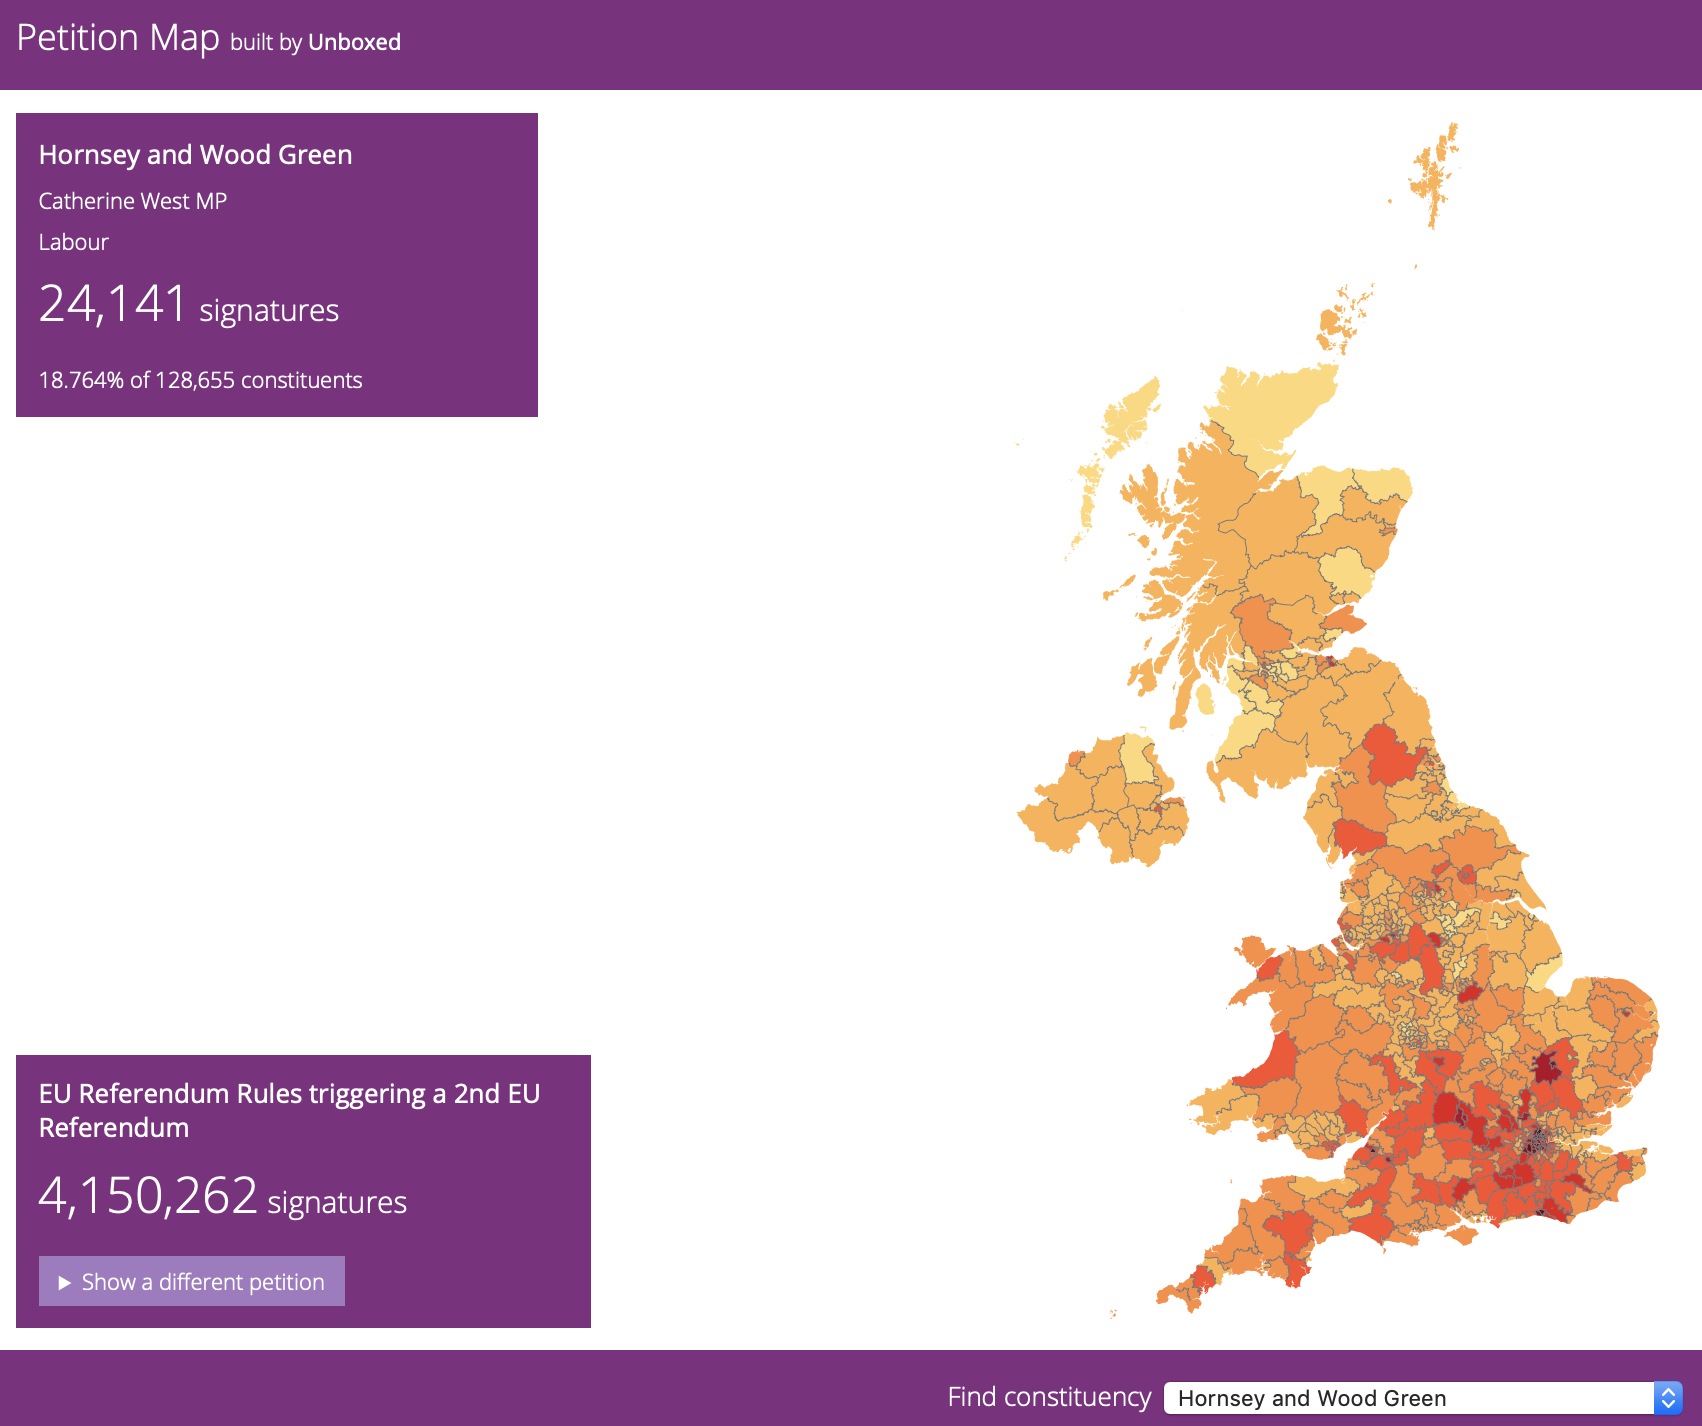
\includegraphics[width = \textwidth]{eu_map.png}
\end{center}
\end{figure}

\section{Summary statistics}

Table \ref{tab:summary_vars} presents descriptive statistics for the main variables used in the participation analysis, and tables \ref{tab:summary_vars_approval} gives the equivalent statistics for the approval analysis. 

\input{tables/summary_statistics.tex} 

\input{tables/summary_statistics_approval.tex} 

\newpage


\section{Descriptive analysis of petition signatures}\label{app:ecological}

Table \ref{tab:constituency_predictors} presents the results for a simple descriptive analysis which documents the variation in aggregate petition signature rates across parliamentary constituencies in the UK. I calculate the total number of signatures per constituency across all petitions in the data that received over 1000 signatures nationally. I then divide this by the number of people living in the constituency in 2015 to get the aggregate number of signatures per capita, and use this as an outcome variable in a linear regression model. The right-hand side variables are demographic -- median pay; percentage female; percentage under 30; population density; percentage of students; percentage working in industry; percentage of home owners; percentage white; percentage unemployed -- or political -- vote for `Leave' in the 2016 UK-EU referendum; Labour, Liberal Democrat, SNP, and `Other' vote share in 2015. In model 2 of table \ref{tab:constituency_predictors}, I also include regional fixed-effects.

\input{tables/constituency_signature_predictors.tex}

The table shows that the volume of signatures that constituencies contribute across petitions vary in predictable ways. Constituencies which have high numbers of young people, lower levels of industrial workers, lower levels of unemployment and which are less ethnically diverse tend to contribute more signatures to e-petitions. Similarly, constituencies in which more people supported `Remain' in the EU referendum are significantly more likely to sign e-petitions. 

\clearpage

\section{Debated petitions}\label{app:debated_petitions}

Table \ref{tab:debated_petitions} presents the titles, total signature counts, and debate dates of all  \input{useful_numbers/n_petitions_wmin_hall.tex}\unskip\ debated e-petitions in the data.

\input{tables/debated_petitions.tex} 
\clearpage
\newpage

\section{Topic control strategy validation}\label{app:topic_validation}

I validate the topic control strategy in three ways. First, if MPs speak predictably on certain issue areas, then models that include topics should have better predictive performance than models without this information. In figure \ref{fig:aic} I show that including MP-specific topic effects clearly decreases the DIC of the model relative to a null model which omits these effects. Furthermore, the model with \input{useful_numbers/best_k.tex}topics performs best in terms of DIC, and I focus on the results from this model throughout the paper. Figure \ref{app:all_topic_model_results} presents the coefficients of interest from all 20 topic models. Regardless of the specific topic model, the results are statistically and substantively very similar.

\begin{figure}[h]
\begin{center}\caption{DIC by topic}\label{fig:aic}
\vspace{-1.5cm}
\includegraphics[width = \textwidth]{figures/dic.pdf}
\end{center}
\end{figure}

\begin{figure}[t]
\begin{center}

\includegraphics[width = \textwidth,frame]{figures/all_topic_model_gamma_coefficients.pdf}

\end{center}
\caption{\label{app:all_topic_model_results} \textbf{Participation results are insensitive to topic-model specification}\\ 
The figure depicts the main second-level coefficients of interest ($\varphi_0$, $\varphi_{\text{Frontbench}}$, $\varphi_{\text{New MP}}$ and $\varphi_{\text{Margin}}$) from equation \ref{eq:gamma_priors} for each of the topic models I estimate. The x-axis of each sub-panel gives the number of topics, and the y-axis gives the value of the relevant coefficient.  Regardless of the number of topics estimated in the CTM model, the results are very similar.}
\end{figure}

Second, table \ref{tab:beta_validation_names} lists the names of 6 MPs with the highest $\beta_{ik}$ coefficients from 4 example topics. The results are encouraging as MPs are associated with topical areas on which we have strong intuitions that they should be active. For example, the listed MPs with the highest coefficients for the ``trade;eu;union;negoti;european'' topic are all well-known campaigners on the issue of the relationship between the UK and the EU and include MPs from both the `Remain' (Hillary Benn, Keir Starmer) and `Leave' (Liam Fox, David Davis, Steven Baker) camps. Similarly, the MPs appearing in the ``nhs;hospit;doctor;patient;amp'' topic also make sense in substantive terms: Jeremy Hunt, Stephen Barclay and Ben Gummer were the Secretary, Minister and Undersecretary of State for Health, respectively, during the time period, and Heidi Alexander and Jon Ashworth have both been the shadow Secretary of State for Health during this period. 


\begin{table}
\caption{MPs with highest $\beta_{ik}$ coefficients by topic}\label{tab:beta_validation_names}
\vspace{-1cm}
\begin{center}
\input{tables/combined_validation.tex} 
\vspace{-.5cm}
\end{center}
\end{table}

Similar patterns hold for the MPs listed under the ``syria;daesh;iraq;syrian;humanitarian'' topic. During the study period, Michael Fallon was the Secretary of State for Defence, and Hilary Benn and Emily Thornberry have both been the shadow Secretary. Similarly, MPs who feature on the ``pupil;school;teacher;academi;educ'' topic held government roles in the Department for Education (Nick Gibb, Edward Timpson) or were members of the opposition front-bench focussed on education (Lucy Powell; Angela Rayner). Overall, these tables reveal that the text-based control strategy I employ has reassuring face validity: the procedure automatically associates MPs with topical areas on which we have strong intuitions to believe they should be active.

Finally, as described in the main text of the paper, the control strategy relies on how well we can approximate the topics of petition debates in the full sample of non-petition debates. To investigate this, table \ref{tab:closest_matching_debates} shows, for each of the petition debates in the data, the titles of the three closest matching \emph{non-petition} debates according to the cosine-similarity between the topic vectors. I calculate the cosine similarity between the topic vectors of each petition debate and every other non-petition debate in the data. I then rank the debates for each petition debate according to this metric and select the top three to display in table \ref{tab:closest_matching_debates}.
Again, the results are reassuring as across almost all petition debates in the sample, the topic model clearly clusters petition debates with non-petition debates that focus on substantively very similar policy areas. 

Linear regression estimates (table \ref{tab:closest_matching_regression_ests}) show that a five-unit increase in the signature rate is associated with an increase of \input{useful_numbers/true_linear_5_point_effect.txt} percentage points in participation probability of petition debates. However, a five-unit increase in the signature rate is also associated with a \input{useful_numbers/closest_linear_5_point_effect.txt} percentage point increase in participation in these closest matching \emph{non-petition} debates. This reinforces the importance of including MP-specific topic effects: MPs are likely to be active on topics that are of greater interest to their constituents, even in the absence of the information provided by an e-petition.

\input{closest_debates/60_topics.tex}

\input{tables/closest_matching_confounding_regression.tex}

Overall, the topic-control strategy improves our ability to predict MP debate participation; associates MPs to topics in ways that are consistent with intuitions about British politics; and links petition-debates to counterfactual non-petition-debates that are very similar in terms of their topical content. 

\clearpage


\section{Alternative independent variable specifications}\label{app:alt_x_spec}

To assess the degree to which the results presented in the body of the paper are sensitive to the specification of the main signature rate variable defined in equation \ref{eq:rel_sig_rate} I present a series of bivariate logistic regression models below in table \ref{tab:x_spec_comparison}. Each model in the table presents the effect of petition signatures on debate participation, but where the exact measure for petition signatures varies across models. In particular, I test each of the following specifications for the signature rate:

\begin{eqnarray}\label{alt_x_rel_sig_rate}
X_{id}^1 &=& \frac{\text{Constituency Signatures Per Capita}_{id}}{\text{National Signatures Per Capita}_d} - 1
\end{eqnarray}

\begin{eqnarray}\label{alt_x_log_rel_sig_rate}
X_{id}^2& = & log\left(\frac{\text{Constituency Signatures Per Capita}_{id}}{\text{National Signatures Per Capita}_d} \right) 
\end{eqnarray}

\begin{eqnarray}\label{alt_x_sigs}
X_{id}^3& = & log\left(\text{Constituency Signatures}_{id}\right)
\end{eqnarray}

\begin{eqnarray}\label{alt_x_sigs_per_cap}
X_{id}^4& = & \text{Constituency Signatures Per Capita}_{id}
\end{eqnarray}

\begin{eqnarray}\label{alt_x_rel_const_sig_rate}
X_{id}^5& = & \frac{\text{Constituency Signatures Per Capita}_{id}}{\text{Average Constituency Signatures Per Capita}_i} - 1
\end{eqnarray}

Equation \ref{alt_x_rel_sig_rate} is the measure I use in the paper, and is included here as a baseline comparison. Equation \ref{alt_x_log_rel_sig_rate} is the log of the signature rate variable used in the paper. Equation \ref{alt_x_sigs} is the log of the number of signatures from a given constituency on a given petition. Equation \ref{alt_x_sigs_per_cap} is the number of signatures from a given constituency on a given petition, divided by the number of electors in that constituency in 2015. Finally, equation \ref{alt_x_rel_const_sig_rate} is the same as equation \ref{alt_x_rel_sig_rate}, but here rather than normalising the signature rate of a given constituency on a given petition by the national signature rate on that petition, I instead normalise by the average constituency rate across all petitions. Finally, for the purposes of comparison, I standardise each of these variables to have a mean of zero and a standard deviation of one.

\input{tables/signature_spec_comparison.tex}

As table \ref{tab:x_spec_comparison} makes clear, regardless of how the signature rate variable is specified, I find a strong, positive, and significant relationship between constituency petition signatures and the probability of debate participation of the relevant MP.

\clearpage

\section{Regression weights for alternative specifications of the signature rate}\label{app:reg_weights}

The specification of the main independent variable in the paper normalises the per-capita signature rate of petition $d$ in constituency $i$ by the national signature rate on petition $d$ in the country as a whole:

\begin{equation}\label{relative_sig_rate}
\text{Signature rate}_{id} = \frac{\text{Constituency Signatures Per Capita}_{id}}{\text{National Signatures Per Capita}_d} - 1
\end{equation}

An alternative approach would be to simply use the numerator of equation \ref{relative_sig_rate}:

\begin{equation}\label{sig_rate}
\text{Constituency Signatures Per Capita}_{id} = \frac{\text{Constituency signatures}_{id}}{\text{Constituency population}_{i}}
\end{equation}

\noindent and include debate fixed-effects on the right-hand side of the model (similar to the $\delta_d$ intercepts I include above). The correlation between these two measures for any given petition will be 1, as equation \ref{relative_sig_rate} is simply equation \ref{sig_rate} normalised by a quantity that is constant within petitions. Given this, and the fact that the model described in the paper includes debate-specific intercepts ($\delta_d$), it might seem intuitive that equations \ref{relative_sig_rate} and \ref{sig_rate} should result in the same substantive inferences for the second-level $\varphi$ parameters that are the main quantities of interest. 

However, re-estimating the main model presented in the paper but substituting equation \ref{sig_rate} for \ref{relative_sig_rate} would, in fact, result in different estimates. The reason that these approaches do not give exactly the same results, even in a model with completely free intercepts for each petition, is that generalised linear models implicitly put larger weight on observations with greater conditional-variance of the treatment \citep{aronow2016does}. In this case, as shown in figure \ref{fig:cond_var}, the debate-level variance of equation \ref{sig_rate} is much larger for those petitions that are marked, on average, by large numbers of signatures. As a consequence, a model using equation \ref{sig_rate} will put very large weights on just a few of the petition debates, and give essentially zero weight to all other petitions. By contrast, there is no relationship between the debate-level variance in equation \ref{relative_sig_rate} and the aggregate number of signatures a petition receives. 

\begin{figure}[h]
\begin{center}\caption{Conditional variance of signature rate variable specifications}\label{fig:cond_var}
\includegraphics[width = \textwidth]{figures/conditional_variance_sig_rate.pdf}
\end{center}
\end{figure}

To demonstrate the consequences that the two specifications of the independent variable would have for the implicit regression weights, I use an approach described in \cite{aronow2016does} which allows me to characterise the effective sample that informs the estimation of the $\varphi$ coefficients in the main model. \cite{aronow2016does} show that the multiple regression weight of unit $i$ will be equal to $(D_i - E(D_i|X_i))^2$, where $D_i$ is the explanatory variable of interest. In other words, we can characterise the contribution of each unit to the estimates of the regression coefficients simply by squaring the residuals of a regression of the treatment variable on the other explanatory variables in the model.\footnote{Although their focus is on linear regression, Aronow and Samii (\citeyear[257]{aronow2016does}) also show that the weights implied by logistic regression (as used here) are approximately equal to those implied by OLS.} 

In this case, the key explanatory variables of interest are the debate-level intercepts ($\delta_d$) in equation \ref{eq:model} in the main body of the paper. Therefore, to characterise the effective sample that informs the estimation of the $\varphi$ coefficients, I regress equation \ref{sig_rate} on debate and MP fixed-effects, square the estimated residuals from that regression, and then take the sum of the weights for each petition debate in the sample. Doing so allows us to see the degree to which any given petition debate contributes to the estimates of the petition-signature effect estimates that are our main focus here.

The full sample consists of 76 petition debates. However, when estimating a model on the basis of equation \ref{sig_rate}, just two of these debates would contribute 88\% of the total multiple regression weight. This implies that the coefficients that are of primary interest in the model -- the $\varphi$ parameters -- would be almost completely informed by just two parliamentary debates were I to use the specification in \ref{sig_rate}. Furthermore, the two debates that receive the vast majority of the weight are clearly atypical with respect to the other petitions discussed in parliament. The first (which accounts for 73\% of the weight) is the debate on holding a second EU referendum (which received four million signatures), and the second (which accounts for 15\% of the total regression weight) is the referendum on President Trump's planned state visit to the UK (which received two million signatures). Furthermore, only 39 of the 76 debates receive a weight that accounts for more than 0.1\% of the total, and only 6 debates have weights that are larger than 0.5\% of the total. Finally, the correlation between the estimated regression weights and the total signature count on each petition is 0.93, implying that the quantities of interest I estimate would be heavily influenced by the most popular petitions.

It would clearly be suboptimal to base inferences on a regression model which relies so heavily on just two fairly extreme examples of the petition debates which I study. The specification I use substantially reduces the degree to which different debates receive different regression weights. For instance, the largest proportional weight for any petition debate in the sample when using equation \ref{relative_sig_rate} is 14\% with all petition debates receiving a weight that is greater than 0.1\% of the total weight, and 49 debates receiving a proportional weight of 0.5\% or above. Furthermore, using the specification in equation \ref{relative_sig_rate} removes the correlation between petition size and regression weights: the correlation is just -0.1 for this variable. Overall, then, it is clear from the analysis presented here that the measure used in the paper provides estimates of the main coefficients of interest that are significantly more representative of the population of debates that I study than would be the case were I to run a model that used the measure described in equation \ref{sig_rate}.

\clearpage

\section{`Tagged' petition debates}\label{app:tagged_petition_debates}

The Petitions Committee can schedule debates on petitions in two distinct ways. The standard way of allocating time to discussion of a petition is to hold a specific debate relating to that petition in a regular session on Monday afternoons in Westminster Hall -- an antechamber of the main House of Commons debating chamber. In the sample I study,   \input{useful_numbers/n_petitions_wmin_hall.tex}\unskip\ of \input{useful_numbers/n_petitions.tex}\unskip\ petitions were scheduled for debate in this manner. The remaining petitions were instead `tagged' to existing House of Commons debates. As the Committee puts it on their website: 

\begin{quote}
``When the House of Commons debates something which is about the issue of a petition, the Petitions Committee can ask for that petition to be ``tagged'' to the debate. If [a] petition is tagged to a debate, it is listed on the order paper (agenda) of the House of Commons as being relevant to the debate. This means MPs know about [the] petition and it can help inform their contributions. Therefore, even if [a] petition is not granted a dedicated debate by the petitions Committee, it can be used by MPs in debates on related topics. Petitions can only be tagged if approved by the sponsor of the debate. The sponsor of the debate can be the Government, the Opposition or a Back Bench MP.'' \citep{committeeWebsite}
\end{quote}

The procedures behind ``tagged'' debates are therefore not the same as those for dedicated petition debates, and they appear to be used on a more ad hoc basis -- it is not even clear that the tagging process always happens before a debate takes place, meaning that MPs are unlikely to be aware of the strength of constituent opinion on an issue.\footnote{Based on personal correspondence with the clerk of the Petitions Committee.} Because of this, the information mechanism I focus on in the paper is likely to be much weaker, and I expect the effects of petition signatures to be much smaller for the ``tagged'' petition debates held in the Commons Chamber than for the dedicated petition debates held in Westminster Hall. 

To investigate this idea, for individuals $i,...,N$, debates $d,...,D$, topics $k,...,K$, and locations $l \in \{1 = \text{Commons Chamber}, 2 = \text{Westminster Hall}\}$, I model debate participation in a hierarchical logistic regression of the following form:

\vspace{-0.5cm}
\begin{eqnarray}\label{eq:model_location}
\text{logit}(y_{id(l)}) =  \alpha_0 + \alpha_{i} + \delta_{d} + \sum_{k=1}^{K}\beta_{ik}\lambda_{kd}  + \gamma_{i,l}  * \text{Signature rate}_{id(l)}%, \sigma_y^2)
\end{eqnarray}

\noindent this model is identical to the model specified in equation \ref{eq:model}, but here $\gamma$ is a \emph{matrix} (rather than a vector) of MP-signature coefficients which consists of two vectors: one for debates held in the Commons Chamber, and one for debates in Westminster hall. The $l$ subscript indicates that I estimate two signature rate coefficients per MP-time period -- one for debates in the Commons' Chamber, and one for debates in Westminster hall -- which allows me to capture the expected heterogeneity across debate settings. 

As in the main analysis, I also model the effect of signatures as a function of MP types:

\vspace{-0.5cm}
\begin{eqnarray}\label{eq:gamma_priors_location}
\gamma_{i,l} \sim N(\varphi_{0_l} + \varphi_{\text{New MP}_l}*\text{New MP}_i + 
\varphi_{\text{Government}_l}*\text{Government}_i + \varphi_{\text{Margin}_l}*\text{Margin}_i, \sigma_{\gamma,l}^2)
\end{eqnarray}

Figure \ref{fig:second_level_double} presents the second-level coefficients from the model (equivalent to figure \ref{fig:subnationalmargins} in the main analysis) with associated 90 and 95\% posterior intervals. Blue points are Westminster Hall coefficients, and black points represent coefficients relating to the Commons' Chamber. Consistent with the argument above, the plot shows that -- regardless of MP characteristics -- the signature-rate has essentially no effect on participation for debates held in the main chamber of the Commons. By contrast, the estimates for the effects of the signature rate in Westminster Hall debates are consistent with those presented in the main body of the paper (table \ref{tab:part_results} and figure \ref{fig:subnationalmargins}).

\begin{figure}[t]
\centering

\includegraphics[width = .5\textwidth]{figures/second_level_slope_coefficients_double.pdf}

\caption{\label{fig:second_level_double} \textbf{Effects of signature rate on debate participation -- ``Tagged'' debates}\\
While there is no relationship between petition signatures and participation in debates in the Commons Chamber (black points), there is a positive relationship between signatures and participation for debates in Westminster Hall (blue points).}

\end{figure}

\clearpage

\section{MP promotion of e-petitions via Twitter}\label{app:twitter}

To investigate the possibility that MPs use social media to drive their constituents to sign e-petitions that address issues on which the MPs are already active, I collect data on the tweets sent by MPs during the 2015-2017 parliamentary term from the Twitter API (\url{https://developer.twitter.com}). Not all MPs have twitter accounts, but I was able to identify the accounts of 554 MPs (out of 650) during this term. I collected all tweets sent by each MP between May 2015 and May 2017, resulting in just over 1 million tweets. I begin by taking a naive approach which almost certainly over-estimates the propensity for MPs to tweet about the petitions system by searching the strings of the tweets for the word ``petition''. Although any tweet about the petition system is likely to include this word, so will many other tweets that are not about the petitions system (such as tweets about local petitions, or petitions run through private organisations such as \href{http://www.change.org}{Change.org}). Even with this permissive search criteria, the numbers of MPs making use of Twitter as a platform for promoting government e-petitions is very small. Of the more than 1 million tweets in my sample, only 1868 include the word ``petition''. Furthermore, of the MPs in my sample, a little over half ever mention petitions.

For a more conservative accounting of MPs' promotion of petitions from the parliamentary petition system, I search the strings of the tweets for links to the official e-petition website.\footnote{These are easily identifiable through the search string ``\texttt{https://petition.parliament.uk/petitions/}''} Again, while some MPs appear to use Twitter to promote e-petitions, the numbers are very small, as only 878 tweets include links to the parliamentary e-petition website. Further, of those MPs for whom I am able to collect Twitter data, only 258 ever include a link to the petitions website in their tweets during the study period. Given these small numbers, it seems highly unlikely that MP activism could explain the substantive results described in this paper.




\clearpage


\begin{table}
\begin{center}

\input{tables/multilevel_model_estimates.tex}


\end{center}

\caption{\label{tab:part_results_full} \textbf{Second-level predictors (debate participation)} \\ Table presents median estimates and associated 95\% posterior intervals for the second-level logit coefficients described in equations \ref{eq:gamma_priors} and \ref{eq:alpha_priors} for the debate participation analysis. Model 1 is a baseline model, models 2 and 3 introduce MP and debate random-effects respectively, and model 4 includes both sets of random effects. Model 5 includes the  matrix of MP-topic random-effects ($\beta_{ik}$). }
\end{table}


\begin{table}
\begin{center}
\input{tables/multilevel_model_estimates_approval.tex}

\end{center}

\caption{\label{tab:approval_results_full} \textbf{Second-level predictors (petition approval)} \\ Table presents median estimates and associated 95\% posterior intervals for the second-level logit coefficients described in equations \ref{eq:gamma_priors} and \ref{eq:alpha_priors} for the petition approval analysis. Model 1 is a baseline model, models 2 and 3 introduce MP and debate random-effects respectively, and model 4 includes both sets of random effects. }
\end{table}

\newpage





\begin{table}
\begin{center}
\input{tables/multilevel_model_estimates_no_party.tex}
\caption{\label{tab:part_results_no_party}\textbf{Second-level $\varphi$ effects (debate participation) -- without party control} \\ The table presents median estimates and associated 95\% posterior intervals for the second-level $\varphi$ coefficients described in equation \ref{eq:gamma_priors}, but here excluding the $\varphi_\text{Party}$ coefficients. }
\end{center}

\end{table}


\clearpage

\section{Qualitative evidence on MPs' knowledge of petition signatures}\label{app:petition_knowledge}

In this section, I present qualitative evidence taken from the texts of petition debates in parliament and use this to emphasise three main points that are relevant to my argument. First, MPs appear to have detailed knowledge of the number of their constituents who sign specific e-petitions. Second, MPs are able to make comparisons about the relative levels of petition support, both across petitions and across constituencies. Third, MPs make frequent references to their role as representatives of their constituents when discussing local petition support. 

Although the quotes presented here do not form a representative sample of all petition debate in the Commons, they nevertheless help to illustrate the knowledge that MPs have of the information contained in specific petitions, and suggest that MPs use this information to guide their representational behaviours in parliament.

First, it is clear from a cursory reading of the petition debates that MPs frequently mention the exact level of support for a given petition amongst their constituents. For example:

\begin{quote}
Nearly 17,500 people in Ealing Central and Acton signed this petition and 72\% of my constituents wanted to remain, so I am here on their behalf.  \\ 
-- Dr Rupa Huq, Labour, \href{https://hansard.parliament.uk/commons/2016-09-05/debates/D2FA95BF-6E07-497D-83A4-0B7341384289/EUReferendumRules}{\emph{EU Referendum Rules}}, 5th September 2016
\end{quote}

\begin{quote}
I understand and share the frustration of my constituents, more than 5,000 of whom signed the petition -- the highest number in Scotland outside Edinburgh, interestingly enough. \\ 
-- Patrick Grady, SNP, \href{https://hansard.parliament.uk/commons/2016-09-05/debates/D2FA95BF-6E07-497D-83A4-0B7341384289/EUReferendumRules}{\emph{EU Referendum Rules}}, 5th September 2016
\end{quote}

\begin{quote}
Some 23,815 people in Bristol West signed this e-petition -- I think that was the second-highest number -- and in the referendum more than 80\% of my constituents voted to remain. \\ 
-- Thangam Debbonaire, Labour, \href{https://hansard.parliament.uk/commons/2016-09-05/debates/D2FA95BF-6E07-497D-83A4-0B7341384289/EUReferendumRules}{\emph{EU Referendum Rules}}, 5th September 2016
\end{quote}

\begin{quote}
I take the opportunity to thank every single one of my constituents who has used the petition to have their voice heard. Just over 3,500 of them have signed the e-petition on preventing Donald Trump's state visit, which amounts to nearly 60 people out of every 1,000 registered voters in Bradford West.\\ 
-- Naz Shah, Labour, \href{https://hansard.parliament.uk/commons/2017-02-20/debates/34847E5C-8B14-46E6-8251-AE99526CC011/PresidentTrumpStateVisit}{\emph{President Trump: State Visit}}, 20th February 2017
\end{quote}


\begin{quote}
The petition has received about 300,000 signatures, of which some 930 were from my Falkirk constituency. That is a declaration, if ever there was one, of people's concern for animal welfare. \\ 
-- John Mc Nally, SNP, \href{https://hansard.parliament.uk/commons/2018-11-26/debates/C95047CD-F24E-44DA-BE73-FC571B014CEF/FireworksPublicSales}{\emph{Fireworks: Public Sales}}, 18th June 2018
\end{quote}


\begin{quote}
I want to thank the \ldots 265,272 members of the public who signed the petition, who include 663 people from my constituency. \\ 
-- Eleanor Smith, Labour, \href{https://hansard.parliament.uk/commons/2017-12-18/debates/D4D9004C-0D4E-4DAD-8C98-309E2C42D2E1/EnslavementOfBlackAfricans(Libya)}{\emph{Enslavement of Black Africans (Libya)}}, 18th December 2017
\end{quote}


Second, beyond simply reporting the numbers of constituents who sign a given petition, MPs also appear to be able to make comparisons of petition support across constituencies:

\begin{quote}
A higher percentage of constituents from Brighton signed the petition than from any other constituency and I am proud to represent them today. \\ 
-- Caroline Lucas, Green, \href{https://hansard.parliament.uk/commons/2017-02-20/debates/34847E5C-8B14-46E6-8251-AE99526CC011/PresidentTrumpStateVisit}{\emph{President Trump: State Visit}}, 20th February 2017
\end{quote}

\begin{quote}
As might be expected, there are a substantial number of signatories to the petition from Staffordshire -- and, indeed, from across the border in south Cheshire. For instance 400 people signed in Crewe and Nantwich and 270 signed in Congleton. There were 458 signatures from my constituency, and Newcastle-under-Lyme, the constituency where I live, came top with 485. \\ 
-- Jeremy Lefroy, Conservative, \href{https://hansard.parliament.uk/commons/2018-07-16/debates/51B3E06E-CDFE-45DD-BD6B-D9B304DA4298/DangerousDogsActStaffordshireBullTerriers}{\emph{Dangerous Dogs Act: Staffordshire Bull Terriers}}, 16th July 2018
\end{quote}

\begin{quote}
When I saw the statistics on this e-petition \ldots Livingston came out top, followed by Linlithgow and East Falkirk, and Falkirk had the fifth-most signatories. Scottish constituencies were more likely to have a higher level of signatories on this issue than on many of the e-petitions I have seen. \\ 
-- Martyn Day, SNP, \href{https://hansard.parliament.uk/commons/2018-11-26/debates/C95047CD-F24E-44DA-BE73-FC571B014CEF/FireworksPublicSales}{\emph{Fireworks: Public Sales}}, 18th June 2018
\end{quote}


Likewise, MPs also demonstrate their awareness of how local support for petitions varies within constituencies across issues:

\begin{quote}
My constituents who have signed the petitions have made their views equally clear. Just short of 1,000 people from Mansfield and Warsop signed the petitions in support of a clean Brexit on world trade terms, while only 150 signed the petitions in favour of a second referendum or of stopping Brexit.  \\ 
-- Ben Bradley, Conservative, \href{https://hansard.parliament.uk/commons/2019-01-14/debates/694BA27D-566E-4F52-BC4B-8FC1ACA3F109/LeavingTheEU}{\emph{Leaving the EU}}, 14th January 2019
\end{quote}


\begin{quote}
584 of my constituents have signed the petition, which is really high for my constituency. \\ 
-- Sharon Hodgson, Labour, \href{https://hansard.parliament.uk/commons/2018-11-26/debates/C95047CD-F24E-44DA-BE73-FC571B014CEF/FireworksPublicSales}{\emph{Fireworks: Public Sales}}, 18th June 2018
\end{quote}


\begin{quote}
The petition received 431 signatures from my constituency, which makes it the second most popular in my area. It is second only to the petition on fireworks. \\ 
-- Martyn Day, SNP, \href{https://hansard.parliament.uk/commons/2019-02-11/debates/E0FFB632-2FCA-4341-A9E1-CA6CFAE6BCEF/SecondarySchoolOpeningHours}{\emph{Secondary School Opening Hours}}, 11th February 2019
\end{quote}

Finally, a frequent theme that marks the speeches of MPs in many petition debates is directly related to the concept of dyadic representation. That is, in many cases MPs combine information about the strength of support for a petition in their constituencies with claims that, by participating in the relevant debate, they are representing those who signed the petition:

\begin{quote}
I do not normally speak on foreign policy matters, but I feel duty-bound to speak because so many of my constituents have signed the petition. \\ 
-- James Cartlidge, Conservative, \href{https://hansard.parliament.uk/commons/2017-02-20/debates/34847E5C-8B14-46E6-8251-AE99526CC011/PresidentTrumpStateVisit}{\emph{President Trump: State Visit}}, 20th February 2017
\end{quote}

\begin{quote}
It is a great honour to stand here and represent the 177 people from my constituency who signed the petition and who, like me, believe that a ban on the sale of animal fur in this country needs to be implemented soon.\\ 
-- Giles Watling, Conservative, \href{https://hansard.parliament.uk/Commons/2018-06-04/debates/8F9B6212-E631-4151-ABA7-AED8560CBBEB/FurTrade}{\emph{Fur Trade}}, 4th June 2018
\end{quote}

\begin{quote}
I am pleased to say that 153 people in my constituency of Morley and Outwood have signed this petition and agree with me that we need a ban on the farming of wild animals in tiny wire cages, as it is demonstrably inhumane. \\ 
-- Andrea Jenkyns, Conservative, \href{https://hansard.parliament.uk/Commons/2018-06-04/debates/8F9B6212-E631-4151-ABA7-AED8560CBBEB/FurTrade}{\emph{Fur Trade}}, 4th June 2018
\end{quote}

\begin{quote}
I thank the 331 people in my constituency who signed the petition \ldots and I am pleased to be speaking on their behalf in calling for action on public sector pay.\\ 
-- David Linden, SNP, \href{https://hansard.parliament.uk/commons/2017-12-04/debates/B20D70FA-4B48-4680-B680-0528E9B42474/PublicSectorPay}{\emph{Public Sector Pay}}, 4th December 2017
\end{quote}

\begin{comment}

\begin{quote}
I \ldots thank the 116 constituents of the centre of the universe that is Glasgow East who signed the petition. \\ 
-- David Linden, SNP, \href{https://hansard.parliament.uk/Commons/2018-06-18/debates/37FAA193-1A7C-4FD9-9F12-3275460784D4/HouseOfLordsAbolition}{\emph{House of Lords Abolition}}, 18th June 2018
\end{quote}


\begin{quote}
This debate has arisen in response to a petition signed by more than 115,000 people, including 922 from my constituency. \\ 
-- Julie Cooper, Labour, \href{https://hansard.parliament.uk/commons/2016-11-28/debates/712C7DA1-FBB4-4D7B-BB01-BDB78C66AB89/ChildCancer}{\emph{Child Cancer}}, 28th November 2016
\end{quote}

\begin{quote}
The petition was signed by 442 of my constituents, and I was proud to join 200 of them outside Warrington Hospital in February to protest against NHS privatisation. \\ 
-- Faisal Rashid, Labour, \href{https://hansard.parliament.uk/commons/2018-04-23/debates/A43878B7-E1E8-4205-A7D2-6624BCF0E403/PrivatisationOfNHSServices}{\emph{Privatisation of NHS services}}, 23rd April 2018
\end{quote}

\end{comment}

\clearpage

\section{Variational inference/HMC comparison}\label{app:vi_mcmc}

The main advantage of using variational inference is that it enables the estimation of complicated models that would computationally impossible using typical methods of full Bayesian estimation such as Gibbs sampling. As Grimmer (2011, 37) 

suggests, ``variational approximations are best suited to problems where properties of the posterior make application of a Gibbs sampler difficult or models where many thousands of parameters and complicated sampling steps make convergence of an MCMC methods slow and difficult to assess.'' This is a fitting description of the models estimated in this paper.  

However, one potential concern that arises from the variational inference strategy is that VI tends to understate the degree of uncertainty associated with model coefficients (Blei et al. 2017, Grimmer 2011).\footnote{\emph{Over}stating the degree of uncertainty is less concerning from a substantive perspective but, though less common, this has also been documented in other applications of the VI approach.} This underestimation will particularly occur when there is posterior correlation in parameter values, which with a linear model will arise when the covariate variables are themselves highly correlated. In this instance, the highest pairwise correlation between the key covariates at the second-level of the model -- the Margin, Frontbench, New MP, and party variables -- is just 0.3, implying that large posterior correlation of the estimated $\varphi$ values is therefore unlikely. As a consequence, although the standard errors may be somewhat smaller using VI than a more traditional estimation approach, discrepancies should be relatively small. 

Beyond this indirect evidence, we can also assess whether understating this uncertainty would be likely to substantially affect the conclusions presented in the main paper. In this section, I compare the estimated credibility intervals for key model coefficients that arise from VI to those from a more traditional approach -- Hamiltonian Monte Carlo (HMC) -- which is not subject to such problems.  

HMC cannot be feasibly implemented for the full model which includes MP-topic coefficients ($\beta$ in equation \ref{eq:model}) and so instead I compare estimates from a simpler model which includes MP and debate intercepts ($\alpha_i$ and $\delta_d$) but which excludes MP-topic effects at the first level. I estimate this model twice -- once with VI and once with HMC -- and provide comparisons between these approaches below.\footnote{I also estimate the HMC model in Stan \citep{carpenter2016stan}.}

The key quantity of interest for this analysis is the width of the 95\% credibility intervals for each of the second-level $\varphi$ parameters described in equation \ref{eq:gamma_priors}. The left-hand panel of figure \ref{fig:vi_mcmc} compares the width of these intervals under VI and HMC. The plot presents the ratio of the 95\% credible intervals from the variational approach to the 95\% intervals from the HMC approach. If the credible intervals were equal, then the points would fall on top of the dotted horizontal line, and this would imply that the uncertainty associated with the variational inference estimates was the same as that for the HMC estimates. However, all points but one are below the horizontal line, implying that VI does indeed understate posterior variability in this case. On average, the 95\% VI credibility intervals are only  \input{useful_numbers/vi_percent_of_mcmc_width.txt}\% the width of those constructed using HMC, which is consistent with similar comparisons in other settings (Grimmer 2011, 37).

\begin{figure}[h]
\caption{Variational inference vs HMC coefficients}\label{fig:vi_mcmc}
\includegraphics[width = \textwidth]{figures/vi_mcmc_comparison_plot.pdf}
\end{figure}

In order to assess whether this has consequences for the conclusions drawn from the analysis, the right-hand panel of figure \ref{fig:vi_mcmc} depicts the coefficients and 95\% intervals from the full model presented in the paper (model 5 in table \ref{tab:part_results}) along with a set of `adjusted' 95\% intervals which simply multiply the original intervals by the degree of under-statement associated with the relevant variables in the left-hand figure. In essence, this comparison assumes that the degree of over-confidence demonstrated in this simpler model would translate to the degree of over-confidence from using VI on the main model in the paper. Under this assumption we can ask whether the conclusions drawn in the paper would have been different had I employed HMC rather than VI.

The plot clearly suggests that the use of VI does not change the substantive findings of the paper. In particular, for the $\varphi_0$, $\varphi_\text{Margin}$, $\varphi_\text{Frontbench}$, and $\varphi_\text{New MP}$ coefficients, the 95\% intervals for both the VI and HMC procedures exclude 0. Although the HMC intervals for the $\varphi_\text{Labour}$ coefficient overlap with zero where the VI intervals do not, this coefficient is included as a control in the model and therefore this does not affect any of the substantive claims made in the paper.

Overall, the two plots presented in figure \ref{fig:vi_mcmc} suggest that while the VI procedure does underestimate the uncertainty associated with these coefficients to some degree, none of the substantive results presented in the paper are sensitive to the use of VI as an estimation procedure.


\end{document}
